\chapter{实验几何}

几何学是研究“空间”的形体和性质的科学。“空间”
就是我们和万物以至星象天体共存的所在。在日常生活中,
我们举目四望所见到的地方,都是空间的一部分。同学们在
小学数学课中学过的柱体、锥体、球体等等,它们都各自占
有空间的一部分,并且构成不同的形体。各种形体的种种性
质,如各部分的长度、角度、面积,以及体积等等。都是在
我们的生活和生产实践中所不可缺少的知识。
\begin{figure}[htp]
	\centering
\begin{tikzpicture}[scale=.7]
\begin{scope}
	\draw (1.5,0) ellipse [x radius=1.5, y radius=.5];
	\shade (0,0) rectangle (3,4);
	\shade (1.5,4)[draw] ellipse [x radius=1.5, y radius=.5];
	\draw (0,0)--(0,4);
	\draw (3,0)--(3,4);
		\node at (1.5,-1.5){圆柱};

\end{scope}
\begin{scope}[xshift=5.5cm]	
	\shade (1.5,0)[draw] ellipse [x radius=1.5, y radius=.5];
		\fill[gray!50] (0,0)-- (3,0)--(1.5,4)--(0,0);
		\draw (0,0)--(1.5,4)-- (3,0);
	

	\node at (1.5,-1.5){圆锥};
\end{scope}
\begin{scope}[xshift=12cm]
		\shade [draw, ball color =gray!20] (0,2) circle(2);
	\node at (0,-1.5){球};
\end{scope}
\end{tikzpicture}	
	\caption{}
\end{figure}

自古以来,人们经过实践、观察、分析,已总结出一
系列的有关空间方面的知识,例如,从中国、埃及、巴比
伦、玛雅等古文明中,可以看出对空间的知识都已掌握得
相当丰富了。对于空间知识有系统的研究,从西方的古文
明中可知,起始于古埃及和巴比仑,而在古希腊得到蓬勃
的发展,获得较辉煌的成就。大体说来,古希腊在空间知
识方面的成就,由欧几里得集其大成于他所著的《几
何原
本》\footnote{欧几里得(Euclid约公元前300年左右)所著此书原名Elements, 
	我国明代数学家徐光启(公元1562---1633)把书中部分几何内容
	译成中文定名为“几何原本”。“几何学”这个中文的名称即来源于
	此。}这部书中。在这部书里,欧儿里得把当时所知道的几何
知识经过整理,建立起一个初步完整的理论体系,使这部书反
映出几何学是一门偏重于推理、论证的高度理论性的科学。
但是,和任何其它科学一样,几何学的理论基础也是建
立在实验所得的一些基本事实之上的。在这一章里,我们就
通过实验、观察、归纳来研究所得到的知识,为以后进一
步学习论证几何作准备。

\section{点、直线和平面}
点、直线和平面是空间最简单的,也是最基本的图形。
同学们在日常生活中,对它们早已有直观的认识了。在这一
节里,我们再对它们的本质和相互关系作进一步的分析,确
立点、直线和平面这三个基本的几何概念,并总结点、直线
和平面之间相互关系方面的一些基本性质。

\subsection{点和直线}
在空间,最原始的,也是最基本的概念就是“位置”。
通常,我们就用“点”来标记“位置”。例如在一张地图
上,我们就以小圆点来标记各地的位置(见图1.2).你
可能发现,在地图上北京用“$\bigstar$”,南京用“$\bigcirc$”印制
的,这只是为了把首都和地方城市区别开来。其实,北京、
南京的。“位置”与地图上印制的图形“$\bigstar$”或“$\bigcirc$”的形状
和大小是没有关系的。这样,仅仅考虑“位置”,的图形就是
点。在天象图上也是以小圆点来标记各星体的位置的(见图1.3)

\begin{figure}[htp]\centering
    \begin{minipage}[t]{0.48\textwidth}
    \centering
\includegraphics[scale=.6]{fig/1-2.png}
    \caption{}
    \end{minipage}
    \begin{minipage}[t]{0.48\textwidth}
    \centering
	\includegraphics[scale=.14]{fig/1-3.png}
    \caption{}
    \end{minipage}
    \end{figure}



在几何学的讨论中,我们用不同的大写字母$A,B,C,\ldots$
表示不同的点,如图1.4中的五个点,就在点旁分别标记
以$A$、$B$、$C$、$D$、$E$, 并分别读作点$A$、点$B$、点$C$、点
$D$、点$E$。

\begin{figure}[htp]\centering
    \begin{minipage}[t]{0.48\textwidth}
    \centering
\begin{tikzpicture}[>=latex, scale=.7]
   \tkzDefPoints{.5/1.5/A, -2/.2/B, -1/-1.5/C, 1/-1/D, 2/.2/E, 0/0/O}

\tkzDrawPoints(A,B,C,D,E)
\tkzLabelPoints[left](B,C)
\tkzLabelPoints[right](A,D,E)
    \end{tikzpicture}
    \caption{}
    \end{minipage}
    \begin{minipage}[t]{0.48\textwidth}
    \centering
      \includegraphics[scale=.75]{fig/1-5.png}
    \caption{}
    \end{minipage}
    \end{figure}


在日常生活中,我们经常需要从一个地方走到另一个地
方。例如,同学们早起上学,就得由自己的家所在的位置走
到学校所在的位置。因此,在空间第二个原始的基本概念就
要算是“通路”了。所谓“通路”,就是从一个位置移到
另一个位置的路线。通常在地图上,我们用线来标记各地之
间的种种通路,如铁路、公路等。在几何学的讨论中,“线”
就是表示通路的。它的直观含义就是:一个“动点”由一
个位置移动到另一个位置所走过的“路线”。如图1.5所
示,设$A$、$B$两点分别表示空间的两个位置,那么连结$A$、$B$
两点的可能通路是很多很多的。

在通常情况下,大家都希望所要走的通路愈短愈好,所
以很自然的问题就是:

“在所有连结$A$、$B$两点的各种通路中,哪一条通路最
短?”

光线的存在,直截了当地显示给我们下述空间的基本性
质:

“连结A、B两点的最短通路唯一存在,它就是连结$A$、
$B$两点的\textbf{直线段}”(在均匀介质中,光走直线\footnote{由光学实验,我们知道光线其实走着最省时间的通路,而并不
	是走着最短的通路,再者,光的速度是随着“介质”而定的,例如在
	真空中走的最快,在空气中速度则稍慢(愈稀薄则其速度愈近于真空
	者),在水中则速度更慢,因为通常我们总是在均匀介质中观察光
	线,所以光线的速度是个不变的常数。这样,最省时间的通路也就是
	最短的通路。这就是我们常见常用的事实:光线在均匀介质中走直
	线。})。

\begin{figure}[htp]
	\centering
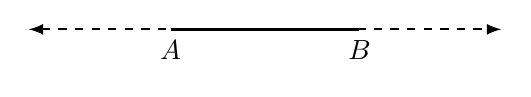
\begin{tikzpicture}[>=latex]
\draw[<->, dashed, thick](-3,0)--(3,0);
\draw[very thick](-1.2,0)node[below]{$A$}--(1.2,0)node[below]{$B$};
\end{tikzpicture}
	\caption{}
\end{figure}


如图1.6所示,由$A$点射向$B$点的光线可以由$A$向$B$的方
向无限延伸;而由$B$点射向$A$点的光线也可以由$B$向$A$的方向
无限延伸,所以对于空间任意两点$A$、$B$, 不但存在着唯一
的最短通路“直线段$AB$”,而且也唯一地确定了一条把直线
段$AB$两端无限延长的直线,这条直线就叫做由$A$、$B$两点所
确定的\textbf{直线},通常称为“直线$AB$”,而直线段$AB$是直线$AB$
介于A、B两点之间的那一段。

归纳上面的讨论,我们可以作出如下的总结:

\begin{enumerate}
	\item “位置”和“通路”是两个最原始的空间概念。
在几何学中,以点表示位置,以线表示通路。
\item 对于任何两点$A$、$B$, 在所有连结、$AB$的可能通路
中,存在唯一的最短通路,就是连结$A$、$B$两点的直线段。
\end{enumerate}

直线段$AB$也简称线段$AB$, 以后我们用符号$\overline{AB}$表示线段
$AB$。点$A$, 点$B$叫做线段$AB$的\textbf{端点}。有时,一条线段也可以
用一个小写字母来表示,例如线段$a$、线段$b$等(图1.7(1))。

\begin{figure}[htp]
	\centering
\begin{tikzpicture}
\begin{scope}
	\draw[|-|](0,0)node[left]{$A$}--(3,0)node[right]{$B$};
\draw[|-|](0,-1)--node[above]{$a$}(1.5,-1);
\draw[|-|](0,-2)--node[above]{$b$}(3,-2);
\node at (1.5,-2.5){(1)};
\end{scope}
\begin{scope}[xshift=6cm]
	\draw[|-|](0,0)node[left]{$A$}--(3,0)node[right]{$B$};
	\draw[|-|](0,-1.5)node[left]{$A'$}--(3,-1.5)node[right]{$B'$};
	\node at (0,-2){$(A)$}; \node at (3,-2){$(B)$};
	\node at (1.5,-2.5){(2)};
\end{scope}
\begin{scope}[yshift=-4cm]
	\draw[|-|](0,0)node[above]{$A$}--(3,0)node[above]{$B$};
	\node at (1.5,-2.5){(3)};
	\draw[|-|](0,-1.5)node[above]{$A'$}--(3,-1.5)node[above]{$B$};
	\draw[|-|](3,-1.5)--(4,-1.5)node[above]{$B'$};
	\node at (0,-2){$(A)$};
\end{scope}
\begin{scope}[xshift=6cm, yshift=-4cm]
	\draw[|-|](0,0)node[above]{$A$}--(3,0)node[above]{$B$};
	\node at (1.5,-2.5){(4)};
	\draw[|-|](0,-1.5)node[above]{$A'$}--(2,-1.5)node[above]{$B'$};
	\draw[|-|](2,-1.5)--(3,-1.5)node[above]{$B$};
	\node at (0,-2){$(A)$};
\end{scope}
\end{tikzpicture}
	\caption{}
\end{figure}

把$\overline{AB}$放在$\overline{A'B'}$上面,使点$A$和点$A'$重合,$\overline{AB}$沿着
$\overline{A'B'}$方向落下,那么有以下三种可能情况:
\begin{enumerate}
	\item 点$B$和点$B'$重合,这时$\overline{AB}=\overline{A'B'}$ (图1.7(2));
	\item 点$B$落在$A'$和$B'$之间,这时$\overline{AB}<\overline{A'B'}$ (图1.7(3));
	\item 点$B$落在$\overline{A'B'}$的延长线上,这时$\overline{AB}>\overline{A'B'}$ (图1.7(4)).
\end{enumerate} 


有一根拉直的绳子$\overline{AB}$, 如果把它分成长度相等的两段。
但是不许用尺来量,应怎么办?

同学们一定会想到,把绳子$\overline{AB}$
的两端点$A$、$B$重叠在一起,并且把绳子拉直,那么在绳子的中间就折出一
个$C$点来(图1.8(2)), 而被折成
的两段绳子$\overline{AC}$和$\overline{CB}$恰好长度相等,这就是说$C$点把$\overline{AB}$平分
了。所以我们把平分线段的点叫做\textbf{线段的中点}。如果点$C$是
$\overline{AB}$的中点,则$\overline{AB}=2\overline{AC}=2\overline{CB}$.

\begin{figure}[htp]\centering
    \begin{minipage}[t]{0.48\textwidth}
    \centering
\begin{tikzpicture}[>=latex, scale=1]
	\draw (0,0)node[above]{$A$}--(3,0)node[above]{$B$};
	\draw (0,-1)node[below]{$A$}--(1.5,-1)node[below]{$C$};
	\draw [dashed](1.5,-1)--(3,-1)node[below]{$B$};
	\node at (4,0){(1)};\node at (4,-1){(2)};
    \end{tikzpicture}
    \caption{}
    \end{minipage}
    \begin{minipage}[t]{0.48\textwidth}
    \centering
    \begin{tikzpicture}[>=latex, scale=1]
      \draw(0,0)node[left]{$A$}--(5,0)node[right]{$B$};
\tkzDefPoints{1/0/M, 2/0/C, 3.5/0/N}
\tkzDrawPoints(M,C,N)
\tkzLabelPoints[above](M,N)
\tkzLabelPoint[below](C){$C$}
\draw[|<->|, dashed](0,-1)--node[fill=white]{24厘米}(5,-1);


    \end{tikzpicture}
    \caption{}
    \end{minipage}
    \end{figure}



\begin{example}
	已知$\overline{AB}=24$厘米,点$C$在$\overline{AB}$上,点$M$、$N$分别是
	$\overline{AC}$和$\overline{CB}$的中点,求$\overline{MN}$的长度(见图1.9)。
\end{example}

\begin{solution}
\[\begin{split}
	\overline{MN}&=\overline{MC}+\overline{CN}=\frac{1}{2}\overline{AC}+\frac{1}{2}\overline{CB}\\
	&=\frac{1}{2}\left(\overline{AC}+\overline{CB}\right)=\frac{1}{2}\overline{AB}=12\text{厘米}
\end{split}\]
\end{solution}

\begin{enumerate}\setcounter{enumi}{2} 
	\item 线段可以向两端无限延长,这样就得到一条直线。一条直线可以用表示它上面任
	意两点的大写字母来表示,如直线$CD$. 有时为了简便,也可
	以在这条直线旁标以一个小写字母,如$\ell$,表示成
	直线$\ell $ (图1.10)。
	\item 对于任何两点$A$、$B$, 都存在着唯一一条通过$A$、$B$
	的直线。这个性质就简述为:\textbf{两点确定一条直线}。
\end{enumerate}

\begin{figure}[htp]
	\centering
\begin{tikzpicture}
\draw (0,0)--(5,0)node[right]{$\ell$};
\tkzDefPoints{1.5/0/C, 3.5/0/D}
\tkzDrawPoints(C,D)
\tkzLabelPoints[below](C,D)
\end{tikzpicture}
	\caption{}
\end{figure}

根据上述性质,我们可以说明其它有关的性质和问题。

\begin{example}
	如果两条直线$\ell$和$m$有一个公共点(交点)$A$(图1.11),它们还能有其它的公共点吗?为什么?
\end{example}

\begin{figure}[htp]
	\centering
	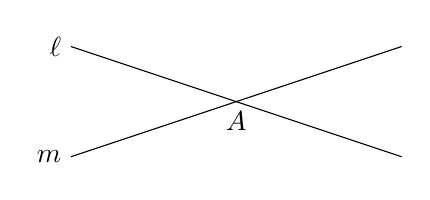
\begin{tikzpicture}[scale=.7]
		\draw (-3,1)node[left]{$\ell$}--(3,-1);
\draw(-3,-1)node[left]{$m$}--(3,1);
\node at (0,0)[below]{$A$};
	\end{tikzpicture}
	\caption{}
\end{figure}

\begin{solution}
除$A$点外,直线$\ell$和$m$不
能再有其它的公共点了。

因为,如
果还有另一个公共点$B$, 那么,$\ell$和$m$就都是通过$A$、$B$两点的直线。
但是通过$A$、$B$两点只有唯一的一条
直线,于是,$\ell$和$m$就是通过$A$、$B$两点的那条唯一的直线,
它们就不是两条不同的直线了。所以,它们除了$A$点外,不
可能再有其它的公共点了。

这件事实可以简述为:\textbf{两条相交直线确定一交点}。
\end{solution}


\begin{example}
	图1.12表示人和物之间放一隔板,使人不能直接
看到物的示意图,$A$表示物,$E$表示人眼,$\overline{BC}$表示隔板。为
了能看见物的形象,放置一面镜子,图中$g$表示镜面,这时
按图1.12(1)中隔板$\overline{BC}$的位置来说,人眼$E$便能看见物A的形象,这是为什么?但按图1.12(2)隔板$\overline{BC}$的位置
来说,人眼$E$便不能看到物$A$的形象,这又是为什么?
\end{example}

\begin{figure}[htp]
	\centering
\begin{tikzpicture}[>=latex]
\begin{scope}
\draw(0.5,0)node[left]{$g$}--(4.5,0);
\draw (1,1)node[above]{$A$}--(2,0)node[below]{$D$}--(4,2)node[right]{$E$};
\draw[dashed] (1,1)--(1,-1)node[below]{$A'$}--(2,0);
\node at (2.5,-2){(1)};
\draw[very thick](3,2.7)node[left]{$B$}--(3,1.2)node[left]{$C$};
\draw[->](1,1)--(1.5,.5); \draw[->](2,0)--(3.5,1.5);
\end{scope}

\begin{scope}[xshift=6cm]
	\draw(0.5,0)node[left]{$g$}--(4.5,0);
	\draw (1,1)node[above]{$A$}--(2,0)node[below]{$D$}--(4,2)node[right]{$E$};
	\draw[dashed] (1,1)--(1,-1)node[below]{$A'$}--(2,0);
	\node at (2.5,-2){(2)};
	\draw[very thick](3,2)node[left]{$B$}--(3,.5)node[right]{$C$};
	\draw[->](1,1)--(1.5,.5); \draw[->](2,0)--(2.5,.5);
	\end{scope}
\end{tikzpicture}
	\caption{}
\end{figure}

\begin{solution}
	按照镜面映象的道理,人眼$E$是从入射线$AD$和反射线$DE$看见$A$的形象的,而点$D$是点$E$和点$A$的象$A'$的连线
	$EA'$和$g$的交点,所以$A$的象$A'$是沿着直线$A'E$映入人眼
	$E$的。因为通过$A'$和$E$只有唯一的一条直线,于是$A'E$和隔板
	$\overline{BC}$不交(图1.12(1))时,在$E$处就看得见$A$的象$A'$, $A'E$和
	$\overline{BC}$相交,也就是被隔板$\overline{BC}$挡住(图1.12(2))时,在$E$处
	便看不见$A$的象$A'$了。
\end{solution}

\begin{example}
	如果在已知$\overline{AB}$上依次取99个点($C_1,C_2,C_3,\ldots,C_{99}$),那么$\overline{AB}$上一共有多少条以这些点为端点的线
	段?($\overline{AB}$也计算在内)
\end{example}	

\begin{solution}
	我们分以下几步来研究这个问题:

	第一,先进行观察、实验。因为每两个点就确定一条线段。因此,
\begin{enumerate}
	\item 在$\overline{AB}$上取一个点$C_1$时,我们看到图1.13(1)中共
	有3条线段$\overline{AB}$、$\overline{AC_1}$和$\overline{C_1B}$.

\begin{figure}[htp]
	\centering
\begin{tikzpicture}[yscale=1.3]
\foreach \x/\xtext in {0/(1),-1/(2),-2/(3),-3/(4),-4.5/(99)}
{
	\draw[|-|] (0,\x)node[below]{$A$}--(8,\x)node[below]{$B$};
	\node at (9,\x){$\xtext$};
}

\draw(2,0)node[below]{$C_1$}--(2,.1);
\draw(1.5,-1)node[below]{$C_1$}--(1.5,-1+.1);
\draw(3,-1)node[below]{$C_2$}--(3,-1+.1);

\foreach \x/\xtext in {1/C_1,2.5/C_2,4/C_3}
{
	\draw(\x,-2)node[below]{$\xtext$}--(\x,-2+.1);
}

\foreach \x/\xtext in {1/C_1,2.5/C_2,4/C_3, 5/C_4}
{
	\draw(\x,-3)node[below]{$\xtext$}--(\x,-3+.1);
}

\foreach \x/\xtext in {1.2/C_1,2/C_2,3.5/C_3,7/C_{99}}
{
	\draw(\x,-4.5)node[below]{$\xtext$}--(\x,-4.5+.1);
}
\node at (4,-3.8){$\vdots$};\node at (9,-3.8){$\vdots$};

\end{tikzpicture}
	\caption{}
\end{figure}

\item 在$\overline{AB}$上取两个点$C_1$、$C_2$时,我们看到图1.13(2)
中共有6条线段$\overline{AB}$、$\overline{AC_1}$、$\overline{C_1B}$、$\overline{AC_2}$、$\overline{C_2B}$和$\overline{C_1C_2}$.
\item 在$\overline{AB}$上取三个点$C_1$、$C_2$、$C_3$时,我们看到图1.13(3)中有10条线段(请同学们自己找出来)。
\end{enumerate}

第二,列表分析找规律
\begin{center}
	\begin{tabular}{cc}
\hline
$\overline{AB}$上取的点数 & $\overline{AB}$上线段的总数\\
\hline
1&3\\
2&6\\
3&10\\
$\vdots$&$\vdots$\\
99& ?\\
\hline
	\end{tabular}
\end{center}

从表上发现:
\begin{itemize}
\item 在$\overline{AB}$上取1个点时,$\overline{AB}$上的线段总数$3=1+2$,
\item 在$\overline{AB}$上取2个点时,$\overline{AB}$上的线段总数$6=1+2+3$,
\item 在$\overline{AB}$上取3个点时,$\overline{AB}$上的线段总数$10=1+2+3+4$。
\end{itemize}

这时,如果在$\overline{AB}$上取4个点,那么$\overline{AB}$上共有多少条线段
呢?由上面发现的规律,可以猜想是$1+2+3+4+5=15$, 数
一下图1.13(4)中的线段数,恰好是15条。这样自然要
问:当在$\overline{AB}$上取99个点时,将会有怎样的结果呢?

第三,归纳、计算

如果在$\overline{AB}$上取99个点,设这时$\overline{AB}$上的线段总数为$S$,
由在第二中发现的规律,不难得出:
\[S=1+2+3+4\cdots +(99+1)=1+2+3+4\cdots +100\]

这是一个很有趣的计算题,如果按顺序加起来,计算是
很麻烦的,我们动动脑筋能否有简便的计算方法呢?

由于$S=1+2+3+\cdots +98+99+100$,也就是:
\[S=100+99+98+\cdots +3+2+1\]
$\therefore\quad 2S=\underbrace{101+101+101\cdots+101+101+101}_{100\text{项}}=100\x 101$

$\therefore\quad S=\frac{100\x 101}{2}=5050$
\end{solution}

\begin{figure}[htp]
	\centering
	\begin{tikzpicture}[scale=.7]
\tkzDefPoints{0/0/B, 6/0/C, 5/3/D, 2/3/A}
\tkzDrawPolygon(A,B,C,D)
\tkzLabelPoints[left](A,B)
\tkzLabelPoints[right](C,D)
\draw(B)--(D);\node at (3.2,1.8)[below]{$O$};
\draw(A)--(C);		
	\end{tikzpicture}
	\caption*{第1题}
\end{figure}

\begin{ex}
\begin{enumerate}
	\item 图中有几条线段,把它们都写出来。
	\item $A$、$B$、$C$三点不在一条直线上,通过其中任何两点画一
	条直线,一共能画出几条直线?
	\item $A$、$B$、$C$、$D$四点中,任何三点都不在一条直线上,通过
	其中任何两点画一条直线,一共能画出几条直线?
	\item 如果$A$、$B$、$C$、$D$、$E$五点中任何三点都不在一条直线
上,通过其中任何两点画一条直线,那么一共能画多少条直线?
	\item 如果有100个点,其中任何三点都不在一条直线上,通
	过其中任何两点画一条直线,那么一共能画多少条直线?
	\item 工人师付在用方砖铺地时,常常打两个木桩,拉线来铺
	砖,这样砖就铺得整齐,这是根据了什么道理?
\item 如果有两个小孩甲、乙在对话,甲问乙:“你的家住在哪
里?”乙回答说:“我的家住在直线$AB$的尽头。”试问
你能沿着直线$AB$找到乙的家吗?为什么?
\item 参看例1.4的归纳、计算,如果在$\overline{AB}$上取$n$个点。那么
$\overline{AB}$上一共有多少条线段?($\overline{AB}$也计算在内)
\item 已知:$\overline{MN}=100$米,$P$点在$\overline{MN}$上,$\overline{MP=45}$米,$S$点是
$\overline{PN}$的中点,求$\overline{PS}$的长度是多少米?
\item 在例1.1中,$\overline{MN}$的长度与$C$点在$\overline{AB}$上的位置有无
关系?
\end{enumerate}
\end{ex}


\subsection{长度的度量}
在给定两点$A$、$B$之间的所有通路之中,以$AB$为最短,
它的“长度”就叫做$A$、$B$\textbf{两点间的距离}。所以,两点间的
距离是连结这两点的线段的长。

长度是我们经常用的一种几何量,现在让我们分别从实
用和数学的观点稍微细致地分析一下“长度”这种几何量的
直观含义,并且谈一谈长度的度量。

一般来说,常用的量基本上可以归成两类:其中一类,例
如一群羊、一堆蛋,它们具有天然的个别单元,即一只羊、一
个蛋。处理这种量,我们只要去数一数它们的“个数”就可以
了。因为它们是可数的。用来数“个数”的数学体系就是我
们在代数学中一开始就详加讨论的自然数系:$\{1,2,3,\ldots\}$. 另一类,例如我们现在要讨论的长度等,这种量虽然不具有
天然个别单元,但是,具有一个基本特点:可以无限细分。
例如,任给一个线段,不管它怎样短,还是可以把它分割成
更短的线段。因此,这种量不可能有天然不可分割的单元,
我们处理这种量的办法就是度量。

因为长度这种量并不具有天然不可分割的单位,所以,
我们只好选用人为的长度单位。例如“米”就是世界上通用
的长度单位。取定长度单位以后,要度量一条线段的长度,
也就是要求得它和长度单位之间的“比值”。例如取定长
度单位为米,所求得的比值是1237:1000,就说这条线段的长
度是1.237米。但是在实践中,这个比值是怎样求出来的
呢?先举几个简单的实例看一看。

\begin{example}
设长度单位是$u$, 所要度量的线段是$a$ (图1.14).
线段$a$恰好可以分割成5段和$u$等长的线段,那么所求的比
值是5, $a$的长度就是$5u$. 

一般地说,如果所要度量的线段$a$恰好可以分割成$m$段
和$u$等长的线段,那末所求的比值就是整数$m$, $a$的长度就是$mu$.
\end{example}

\begin{figure}[htp]\centering
    \begin{minipage}[t]{0.48\textwidth}
    \centering
\begin{tikzpicture}[>=latex, scale=1]
       \draw [|-|](0,0)--(1,0);
	   \draw [|-|](0,-1)--(5,-1);
	   \node at (-.5,0){$u:$};
	   \node at (-.5,-1){$a:$};
	   \foreach \x in {1,2,3,4}
	   {
\draw (\x,-1)--(\x,-.9);
	   }
    \end{tikzpicture}
    \caption{}
    \end{minipage}
    \begin{minipage}[t]{0.48\textwidth}
    \centering
    \begin{tikzpicture}[>=latex, scale=1]
		\draw [|-|](0,0)--(3,0);
		\draw [|-|](0,-1)--(1,-1);
		\node at (-.5,0){$u:$};
		\node at (-.5,-1){$b:$};
		\foreach \x in {1,2}
		{
 \draw (\x,.1)--(\x,0);
		}
    \end{tikzpicture}
    \caption{}
    \end{minipage}
    \end{figure}

\begin{example}
设长度单位是$u$, 所要度量的线段是$b$ (图1.15) 单
位长$u$恰好可以分割成3段和$b$等长的线段,那么所求的比
值是$\frac{1}{3}$, $b$的长度就是$\frac{1}{3}u$. 

一般地说,如果长度单位$u$恰
好可以分割成$n$段和$b$等长的线
段,那么所求的比值是$\frac{1}{n}$
,$b$的长度就是$\frac{1}{n}u$
\end{example}

\begin{example}
	设长度单位是$u$, 所要度量的线段是$c$ (图1.16). $c$比$4u$长些,但又比$5u$短些,如果我们把$u$三等分,
	线段$c$截取4段$u$后所余的一段恰好是$\frac{1}{3}u$的2倍,那么c的
	长度就是$4\frac{2}{3}u$.

\begin{figure}[htp]
	\centering
\begin{tikzpicture}
\draw[|-|] (0,0)node[left]{$b:$}--(4.667,0);
\draw[|-|] (0,1)node[left]{$v:$}--(1,1);
\end{tikzpicture}
	\caption{}
\end{figure}

一般地说,如果把长度单位$u$适当地等分成$n$段,即每
一段$u'$的长度是$\frac{1}{n}\cdot u$, 所要量的线段$c$恰好可以分割成
$m$段和线段$u'$等长的线段,那么$c$的长度就是$\frac{m}{n}u$。

在例1.7中,用长度单位$u$去度量$c$时,怎样才能知道在$c$
上截取4段$u$后,所余的一段恰好是$u$的$\frac{1}{3}$的整数倍?实际上
可以这样来确定:在$c$上截取4段$u$后,以所余的一段$\overline{C_4D}$去
量$u$, 在$u$上截去一段$\overline{C_4D}$后,所余的一段$\overline{U_1V}$又较$\overline{C_4D}$短,
这时再以$\overline{U_1V}$去度量$\overline{C_4D}$, 恰好$\overline{C_4D}$是$\overline{U_1V}$的2倍。这样便
看出$\overline{U_1V}$是$u$的$\frac{1}{3}$,把$u$三等分后,$\overline{C_4D}$就恰好是$\frac{1}{3}u$的2
倍了。
\end{example}

\begin{example}
	设长度单位是$u$, 求线段$d$的长度(图1.17)。
\begin{figure}[htp]
	\centering
\begin{tikzpicture}[xscale=4]
	\draw[|-|] (0,1)node[left]{$u:$}--(1,1)node[below]{$V$};
	\draw[|-|] (0,0)node[left]{$d:$}--(2.42,0)node[right]{$E$};
	\draw(1,0)--(1,.1); \draw(2,0)node[below]{$D_2$}--(2,.1);
	\draw(2.333,0)node[below]{$F_2$}--(2.333,.1);
	\draw(.42,1)--(.42,1.1);  \draw(.84,1.1)--(.84,1)node[below]{$U_2$};
	\draw(2.16,0)--(2.16,0.1);
	\draw(.84+.08,1.1)--(.84+.08,1);
\end{tikzpicture}	
	\caption{}
\end{figure}
\end{example}

\begin{solution}
	在$d$上用圆规截取2段$u$后,所余的一段$\overline{D_2E}$较$u$
短;在$u$上截取2段$\overline{D_2E}$后,所余的$\overline{U_2V}$较$\overline{D_2E}$短;在$\overline{D_2E}$
上截取2段$\overline{U_2V}$后,所余的一段$\overline{F_2E}$较$\overline{U_2V}$短;但$\overline{U_2V}$恰
好是$\overline{F_2E}$的2倍。于是
\[\begin{split}
	\overline{D_2E}&=\overline{D_2F_2}+\overline{F_2E}=2\overline{U_2V}+\overline{F_2E}\\
&=2\cdot 2\overline{F_2E}+\overline{F_2E}=5\overline{F_2E}
\end{split}\]
\[u=2\overline{D_2E}+\overline{U_2V}=2-5\overline{F_2E}+2\overline{F_2E}=12\overline{F_2E}\]
$\therefore\quad \overline{F_2E}=\frac{1}{12}u,\quad \overline{D_2E}=\frac{5}{12}u,\quad d=2\frac{5}{12}u$
\end{solution}


由例1.7和例1.8可以看出,当被度量线段($c$和$d$)不能恰好
被分割而成为长度单位的整数倍,也就是它们不能被长度单
位量尽时,都是求出另一条线段(例1.7中是$\overline{U_1V}$, 例1.8中是$\overline{F_2E}$),使得它能量尽长度单位和被量线段。再按例1.6的方
法求出以长度单位为单位的这条线段的长度,然后便可求出
原来被量线段的长度了。

能够量尽两条线段$a$和$b$的线段,我们叫它做线段$a$和$b$的
\textbf{公度}。两条线段的公度中最长的,叫做\textbf{这两条线段的最大公
度}。$\overline{U_1V}$和$\overline{F_2E}$就分别是线段$u$和$c$, $u$和$d$的最大公度。在
例1.5中线段$u$就是线段$u$和$a$的最大公度;例1.6中的线段$b$就是线
段$u$和$b$的最大公度,象例1.7、例1.8中求线段$u$和$c$、$u$和$d$的最
大公度的方法,叫做\textbf{辗转相截法}。

通过上面各例,我们很自然地会想到:任何两条线段
$a, b$, 它们的长度比值是否总是一个分数(整数也可看作
分数)?换句话说,对于任何两条线段$a$、$b$, 是否存在着它
们的公度?

这个问题从正、反两面来分析它的重要性。首先,如果
任何两条线段的长度的比值总是一个分数,那么分数全体
(即代数开始所讲的有理数)就足以处理长度的度量问题
了。其次,反过来说,如果两条线段的长度的比值不一定是
分数,那么有理数就不足以处理长度的度量问题。因而我们
就得学会一种含有“非分数”的数系才能充分解决度量问
题。这个问题是整个数学发展史上的一件大事,我们以后再
详细讨论。

\begin{ex}
\begin{enumerate}
	\item 已知线段$a$、$b$、$u$, 其中线段$a=9u$, $b=3u$, 问线段$a$、$b$的最大公度是线段$u$的几倍?
	\item 已知线段$a=48$毫米,$b=18$毫米。先用辗转相截法求出
	$a$、$b$的最大公度,并量它等于多少毫米;再用求最大公
	约数的辗转相除法求出48、18的最大公约数。比较前后所得
	的结果。
	\item 根据图形填写下面空白:
\begin{enumerate}
	\item $\overline{AC}=\overline{BC}+(\qquad)$	
	\item	$\overline{CD}=\overline{AD}-(\qquad)$	
	\item $\overline{AC}+\overline{CD}=(\qquad)+\overline{BD}$
\end{enumerate}
\begin{center}
	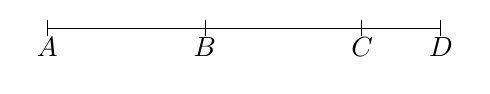
\begin{tikzpicture}
	\draw[|-|](0,0)node[below]{$A$}--(5,0)node[below]{$D$};
	\draw[|-|](2,0)node[below]{$B$}--(4,0)node[below]{$C$};	
	\end{tikzpicture}
\end{center}
\end{enumerate}
\end{ex}

\subsection{直线和平面}
在空间,另一种常见的形象就是各种各样的面。例如地
球的表面,它的整体看起来是一个略为扁平的球面,而局部
的形象又随着当地的地貌而不同。有的地方是一片原,有
的地方是起伏的丘陵,有的地方是一片湖面,也有的地方是
崇山峻岭和深谷。又如教室的一面墙壁,上课用的黑板,以
及桌面等,看起来又都是“平直”的面。

通常检查一个桌面是否“平直”,最简单的方法就是用一
根直尺放在桌面上(图1.18),如果放在任何位置上,直
尺的边都和桌面密合,那么桌面就是“平直”的。我们就说
桌面是平面。但是象图1.19的面上,虽然直尺放在$\ell_1,\ell_2,\ldots,\ell_n$等位置时,直尺边和这个面密合,而在$AB$位置上直尺
边和面就不密合了。这就是说并不是在任何位置上直尺的边
总和这个面密合,这个面不是一个平面,实际上是一个曲
面。
\begin{figure}[htp]\centering
    \begin{minipage}[t]{0.48\textwidth}
    \centering
	\includegraphics[scale=.8]{fig/1-18.png}
    \caption{}
    \end{minipage}
    \begin{minipage}[t]{0.48\textwidth}
    \centering
	\includegraphics[scale=.8]{fig/1-19.png}
    \caption{}
    \end{minipage}
    \end{figure}

在几何学的讨论中,平面就是一个到处平直而且向各个
方向无限延展的面,它的特点就是在它上面任取两点$A$和$B$
(图1.20),直线$AB$就完全在这个平面内。

\begin{figure}[htp]\centering
    \begin{minipage}[t]{0.48\textwidth}
    \centering
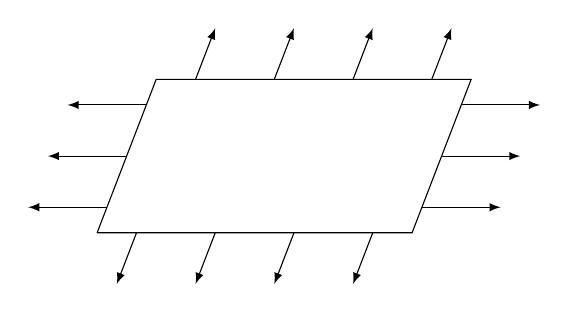
\begin{tikzpicture}[>=latex, yscale=1.5, x={(0:1cm)}, y={(60:.5cm)}]

\draw (0,0)--(4,0)--(4,3)--(0,3)--(0,0);
\foreach \x in {.5,1.5,...,3.5}
{
	\draw[->](\x,0)--(\x,-1);
	\draw[->](\x,3)--(\x,4);
}
\foreach \x in {.5,1.5,2.5}
{
	\draw[->](0,\x)--(-1,\x);
	\draw[->](4,\x)--(5,\x);
}

\tkzDefPoints{1/2.2/A, 2.8/.75/B}
\tkzDrawLine(A,B)
\tkzDrawPoints(A,B)
\tkzLabelPoints[right](A,B)

    \end{tikzpicture}
    \caption{}
    \end{minipage}
    \begin{minipage}[t]{0.48\textwidth}
    \centering
    \begin{tikzpicture}[>=latex, scale=1]
\draw(0,0) rectangle (2,3);
\draw[fill=white](0,0)--(-30:1.8)--+(0,3)--(0,3)--(0,0);
\draw(0,0)--(-140:1.5)--+(0,3)--(0,3);
\draw[dashed,->](0,0)--(0,-1);
\draw[dashed](0,0)--(2,0);
\draw[dashed,->](0,3)--(0,4)node[right]{$\ell$};
\node at (0,1.5)[right]{门轴};
    \end{tikzpicture}
    \caption{}
    \end{minipage}
    \end{figure}

我们观察一扇门,把它看作平面的一部分,那么它的轴
线既在墙壁的平面内(图1.21),又在这扇门所在的平面
内,不可能连结两个“合页”的直线不都在这两个平面内。推动这扇门,它每到一个新的位置都表现了通过轴线的一个平面。这些事实说明了:
\textbf{空间相交的两个平面的“交界”是一条直
线。通过一条直线可有无数个平面。}

\begin{ex}
\begin{enumerate}
	\item 举出一条直线和一个平面没有公共点的实例,以及一条直
	线和一个平面只有一个公共点的实例。
	\item 一点在一平面内,而其它的点都不在这个平面内,这种实例有\item 举出两个平面没有公共点的实例。
	\item 两个平面只有一个公共点的实例存在吗?
	\item 如果空间被平面$\alpha$分成的两部分之一中,有一只小虫子$A$,这只小虫子$A$要爬到	被平面所分空间的另一部分去,假如它
	不穿过平面$\alpha$,能过去吗?为什么?
\begin{center}
	\begin{tikzpicture}
		
	\end{tikzpicture}
\end{center}
\end{enumerate}
\end{ex}

同学们作这样一个实验,张开手指,使拇指、食指和中指的尖
这三点不在一条直线上,拿一张硬纸(它代表一个平
面)往三个指尖上放,看看它是否能同时通过三个指尖?再
拿一张硬纸仍然这样放,看这两张硬纸是否重合?这种特点
对于一个指尖,两个指尖也适合吗?再使母指、食指、中
指,无名指的指尖这四点不在一条直线上,看看能否保证总
有一张硬纸同时通过这四点?仿照“两点确定一条直线”的
特点,同学们能否总结出几个点确定一个平面的结论?

通过上面的实验,我们得出平面的另一个基本性质:
\textbf{空间不共线三点确定一个平面。}

同学们还可进一步思考以下的问题:
\begin{enumerate}
	\item 一直线及直线外一点能确定一个平面吗?
	\item 相交的两条直线能确定一个平面吗?
\end{enumerate}

\section*{习题1.1}
\addcontentsline{toc}{subsection}{习题1.1}
\begin{enumerate}
	\item 什么是线段?什么是直线?两者有什么区别?
	\item 什么是线段的中点?如果有一根笔直的铁棍,
	假如用$\overline{AB}$
	来表示它,不用尺量,也不许把它折弯,你有没有办法找
	出$\overline{AB}$所表示的这根铁棍的中点来?
	\item 请同学们复习一下小学学过的公制、市制两种长度单位,
	并填下表:
	\begin{center}
\begin{tabular}{ll}
	1公里(km)$=\underline{\qquad}$米(m) &\qquad 1里$=\underline{\qquad}$丈\\
1米(m)$=\underline{\qquad}$分米(dm)&\qquad 1丈$=\underline{\qquad}$尺\\
1分米(dm)$=\underline{\qquad}$厘米(cm)&\qquad 1尺$=\underline{\qquad}$寸\\
1厘米(cm)$=\underline{\qquad}$毫米(mm)&\qquad 1寸$=\underline{\qquad}$分
\end{tabular}		
	\end{center}

	\item 	求出下列结果,并化成括号中指定的长度单位:
\begin{enumerate}
\item 5尺4寸5分 $+$ 3尺4寸 $+$ 6尺7寸8分$=\underline{\qquad}$(米);
\item 46厘米 $+$ 1米60厘米 $+$ 7米50厘米$=\underline{\qquad}$(尺);
\item 4丈5尺6寸$\x3=\underline{\qquad}$(米);
\item 5米40厘米$\div 1000=\underline{\qquad}$(毫米);
\item 20mm$\x0.1\%=\underline{\qquad}$(m)
\end{enumerate}

\item 在一条直线上,顺次取$A$、$B$、$C$三点,使$\overline{AB}=4$cm, $\overline{BC}=2$cm, 并且取$\overline{AC}$的中点$O$, 求:
\begin{multicols}{3}
	\begin{enumerate}
		\item $\overline{AO}$的长
		\item $\overline{OB}$的长
		\item $\overline{OC}$的长
	\end{enumerate}
\end{multicols}

\begin{figure}[htp]
	\centering
	\begin{tikzpicture}
	\draw (0,0)--(8,0);
\tkzDefPoints{1/0/A,5/0/B,7/0/C, 4/0/O}
\tkzDrawPoints(A,B,C,O)
\tkzLabelPoints[below](A,B,C,O)	
	\end{tikzpicture}
	\caption*{第5题}
\end{figure}

\item 把一条32cm的线段分成三段,中间的一段长为8cm,问
第一段中点到第二段中点的距离等于多少cm?
\item 图中表明四个点可以确定一条、四条或者六条直线。试
划图说明五个点可以确定1、5、6、8或10条直线(其它情
况不存在)。
\begin{figure}[htp]
	\centering
\begin{tikzpicture}
	\begin{scope}
		\draw (0,0)--(5,0);
		\tkzDefPoints{1/0/P_1,2/0/P_2,3/0/P_3, 4/0/P_4}
		\tkzDrawPoints(P_1,P_2,P_3,P_4)
		\tkzLabelPoints[above](P_1,P_2,P_3,P_4)	
	\end{scope}
	\begin{scope}[yshift=-2cm]
		\tkzDefPoints{1/0/P_2,2/0/P_3,3/0/P_4, 2/-1/P_1}
		\tkzDrawLines[add=.8 and .8](P_2,P_4 P_3,P_1 P_2,P_1 P_1,P_4)
		\tkzDrawPoints(P_1,P_2,P_3,P_4)
		\tkzLabelPoints[above right](P_1,P_2,P_3,P_4)	
	\end{scope}
	\begin{scope}[yshift=-2cm, xshift=6cm]
		\tkzDefPoints{.5/0/P_1,3.5/0/P_3,2/1.5/P_4, 2/-1.5/P_2}
		\tkzDrawLines[add=.5 and .5](P_2,P_4 P_3,P_1 P_2,P_1 P_1,P_4 P_2,P_3 P_3,P_4)
		\tkzDrawPoints(P_1,P_2,P_3,P_4)
		\tkzLabelPoints[above right](P_1,P_2,P_3,P_4)
	\end{scope}
\end{tikzpicture}
	\caption*{第7题}
\end{figure}

\item 在三角形$ABC$的$\overline{BC}$边上如果取$n$个点$P_1,P_2,P_3,\ldots,P_n$,
并把这$n$个点分别和$A$点连结起来,就出现很多三角形,
试研究三角形的总数有多少?(原来的三角形$ABC$也包括
在内)。

(提示:$\overline{BC}$上每一条线段都
可与$A$点构成一个三角形,因此
求三角形的总数实际上就是求
$\overline{BC}$上线段的总数)。
\begin{figure}[htp]
	\centering
\begin{tikzpicture}
	\tkzDefPoints{0/0/B, .5/0/P_1,1.5/0/P_2,3/0/P_n, 4/0/C, 1.5/2/A}
	\tkzLabelPoints[below](P_1,P_2,P_n,B,C)	
	\tkzDrawSegments(A,B A,P_1 A,P_2 A,P_n A,C B,C)
	\tkzLabelPoints[above](A)	
\end{tikzpicture}
	\caption*{第8题}
\end{figure}

\end{enumerate}

\section{方向、角度与平行}
\subsection{方向与角}
当我们在平坦的操场上要从一个位置(以$A$点表示)走
到另一个位置(以$B$点表示),经验告诉我们最省事的走法
是:“由$A$点朝向$B$点一直走”。(图1.22)

\begin{figure}[htp]
	\centering
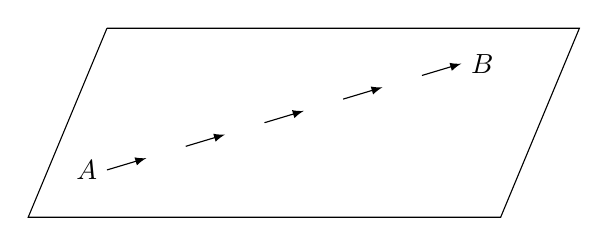
\begin{tikzpicture}[>=latex, yscale=.6]
\draw(1,4)--(7,4)--(6,0)--(0,0)--(1,4);
\draw[->](1,1)node[left]{$A$}--(1.5,1.25);
\draw[->](2,1.5)--(2.5,1.75);
\draw[->](3,2)--(3.5,2.25);
\draw[->](4,2.5)--(4.5,2.75);
\draw[->](5,3)--(5.5,3.25)node[right]{$B$};
\end{tikzpicture}
	\caption{}
\end{figure}

上面这种常用的走法,很明显地突出了“方向”这个常
用的基本几何概念。再设想我们是正在茫茫大海中航行的船
的舵手,或者是一架越洋飞行的飞机的驾驶员,那么“方向”这
个概念就更是至关紧要的了!因为“航行的方向”是我们随
时要确切掌握的要素!

现在让我们就上面的实例,对于所涉及的“方向”这个
概念的直观含义,稍加分析。

假如我们从操场的$A$点走向$B$点去(图1.23),最省事
的“通路”当然就是$\overline{AB}$(因为它是最短的通路)。所以
我们先站在$A$点,向$B$点望一望,头脑中抽象地计画了所要
走的路线应该是直线段(图中虚线所示)。然后便一步步
地沿着设想的路线$\overline{AB}$向$B$点一直走。从几何的观点看,每跨
一步就沿着某一个方向做了一个和自己步幅等长的“有向线
段”。所以说,“由$A$点朝向$B$点一直走的走法”就是每一
步都是沿着$\overline{AB}$这个固定的方向走的那种走法。


\begin{figure}[htp]
	\centering
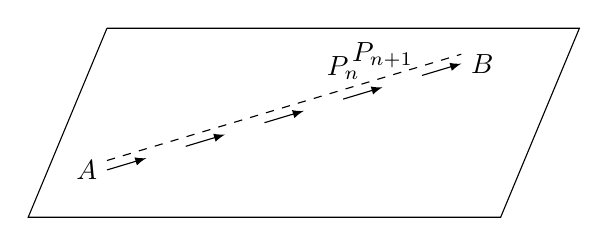
\begin{tikzpicture}[>=latex, yscale=.6]
	\draw(1,4)--(7,4)--(6,0)--(0,0)--(1,4);
	\draw[->](1,1)node[left]{$A$}--(1.5,1.25);
	\draw[->](2,1.5)--(2.5,1.75);
	\draw[->](3,2)--(3.5,2.25);
	\draw[->](4,2.5)--(4.5,2.75);
	\draw[->](5,3)--(5.5,3.25)node[right]{$B$};
	\draw[dashed](1,1.2)--(5.5,3.45);
\node at (4,2.7)[above]{$P_n$};
\node at (4.5,2.95)[above]{$P_{n+1}$};

\end{tikzpicture}
	\caption{}
\end{figure}

在由$A$点可以直接看到$B$点的情形下,要保持每一步的
方向都是正对着$B$点的方向是很简单的。因为我们随时可以用
目光把行进中的位置(图1.23中的$P_n$点)和$B$点连一条直
线,这条直线的方向也就是下一步(图1.23中的$P_nP_{n+1}$)
所要走的方向。但是在另外两个设想的航海和飞行的实例
中,目的地是遥远而看不到的,而计划中要走的航线,所经
过的绝大部分都是“漫无边际”的海洋和天空,毫无可供
“瞄准”的标志。所以要随时保持航行的方向的正确性就变
成确保安全到达目的地的最重要的依据了。

由$A$点出发,沿着一个固定的方向(比如向着$B$点的方
向)前进时,它的路线就是一条\textbf{射线}。如图1.24所示,
它就是居于$A$点右侧的那条半直线。
\begin{figure}[htp]\centering
    \begin{minipage}[t]{0.48\textwidth}
    \centering
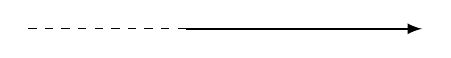
\begin{tikzpicture}[>=latex, scale=1]
       \draw[->, thick](0,0)--(3,0);
	   \draw[dashed](-2,0)--(0,0);
	   \tkzDefPoints{0/0/A,1.5/0/B}
	   \tkzDrawPoints(A,B)
	   \tkzLabelPoints[below](A,B)		   
    \end{tikzpicture}
    \caption{}
    \end{minipage}
    \begin{minipage}[t]{0.48\textwidth}
    \centering
    \begin{tikzpicture}[>=latex, scale=1]
      \draw[->, thick](0,0)node[left]{顶点}--node[below]{边}(4,0);
	  \draw[->, thick](0,0)--node[above]{边}(30:4);
    \end{tikzpicture}
    \caption{}
    \end{minipage}
    \end{figure}

所以我们把直线上一点一旁的部分叫做\textbf{射线},这一点叫
做射线的\textbf{端点}。例如射线$AB$(图1.24)。(注意:表示射
线时,射线的端点字母必须写在前面)。在几何中,我们把
以$A$点为端点的一条射线看作是由$A$点出发的一个方向。

我们把从同一端点引出的两条
射线所组成的图形叫做\textbf{角},这个共同的端点叫做角的\textbf{顶点},这两条射线分别叫做角的\textbf{边}。我们把角看成
是由构成这个角的两条射线所表示的方向差(图1.25)。

一个角通常用符号“$\angle$”(读作角)后边带三个大写字
母来表示,中间一个字母表示角的顶点,两旁的两个字母分
别表示角的两边上的任意点,如图1.26(1)中的角可记作
$\angle AOB$, 读作“角$AOB$”。如果用一个点作顶点的角只有
一个,这个角也可以只用表示顶点的那个大写字母来表示,
如图1.26(1)的$\angle AOB$也可表示为$\angle O$。有时,为了方
便,还可以在角的里面靠近顶点写个数字、或小写希腊字
母表示角,如图1.26(2)(3)中的$\angle 1$、$\angle 2$、$\angle 3$和$\angle \alpha$、$\angle \beta$、$\angle \gamma$等。

\begin{figure}[htp]
	\centering
\begin{tikzpicture}[scale=2]
\begin{scope}
\draw(-1,.5)node[left]{$A$}--(0,0)node[right]{$O$}--(-1,-.5)node[left]{$B$};
\node at (-.5,-1){(1)};
\end{scope}
\begin{scope}[xshift=1.3cm]
	\tkzDefPoints{0/.5/O, -1/-.5/A, -.5/-.7/B, .5/-.7/C, 1/-.5/D}
	\tkzDrawSegments(O,A O,B O,C O,D)
	\tkzMarkAngles[mark=none, size=.4](A,O,B C,O,D)
	\tkzLabelAngle[pos=.5](A,O,B){1}
	\tkzLabelAngle[pos=.5](B,O,C){2}
	\tkzLabelAngle[pos=.5](C,O,D){3}
	\tkzMarkAngles[mark=none, size=.3](B,O,C)
	\node at (0,-1){(2)};
\end{scope}
\begin{scope}[xshift=3.5cm]
	\tkzDefPoints{0/0/O, -1/.5/A, 1/-.5/B, 1/.5/C, -1/-.5/D}
	\tkzDrawSegments(A,B C,D)
	\tkzMarkAngles[mark=none, size=.2](C,O,A D,O,B)
	\tkzMarkAngles[mark=none, size=.3](A,O,D)
	\tkzLabelAngle[pos=.3](D,O,B){$\gamma$}
	\tkzLabelAngle[pos=.4](A,O,D){$\beta$}
	\tkzLabelAngle[pos=.3](C,O,A){$\alpha$}
	\node at (0,-1){(3)};
\end{scope}
\end{tikzpicture}
	\caption{}
\end{figure}

当一个角的两条边重合时,其夹角显然为$O$(即方向
没有差别)。另外一种特殊情形是当角的一边是另一边的反
向延长线时,就称这个角为\textbf{平角}。
如图1.27中射线$CA$和射线$CB$的
方向相反,那么$\angle ACB$就是一个平角。

\begin{figure}[htp]\centering
    \begin{minipage}[t]{0.48\textwidth}
    \centering
\begin{tikzpicture}[>=latex, scale=1]
\draw[<->](0,0)--(5,0);
\tkzDefPoints{1/0/B,2.5/0/C,4/0/A}
		\tkzDrawPoints(A,B,C)
		\tkzLabelPoints[below](A,B,C)	
		\draw[->](3,0) arc (0:180:.5);
    \end{tikzpicture}
    \caption{}
    \end{minipage}
    \begin{minipage}[t]{0.48\textwidth}
    \centering
    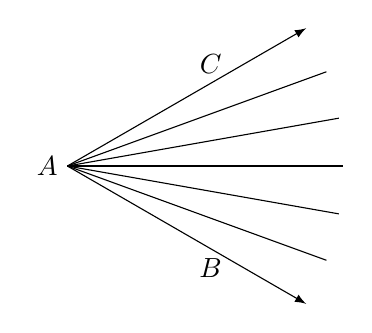
\begin{tikzpicture}[>=latex, scale=.7]
    \foreach \x in {-20,-10,...,20}
	{
		\draw(0,0)--(\x:5);
	}
	\draw[->](0,0)node[left]{$A$}--(30:5);
	\draw[->](0,0)--(-30:5);
\node at (30:3)[above]{$C$};
\node at (-30:3)[below]{$B$};
    \end{tikzpicture}
    \caption{}
    \end{minipage}
    \end{figure}

根据上述,我们可以把日常常用的“方向”和角这两个
概念,给以如下的说明:
\begin{enumerate}
\item 自定点$A$出发的所有方向和以$A$点为端点的所有
射线之间一一地相对应。换句话说,对应于自$A$点出发的一
个方向,就有唯一的一条射线(它就是自$A$点出发沿着这个
固定方向一直走的路线);反之任何一条以$A$点为端点的射
线也就唯一地表示了一个确定的方向。所以在几何学中,我
们以一条射线表示一个方向。
\item 一条以$A$为端点的射线,由起始的任何一小段唯
一确定(因为整个射线只是那一小段沿着那个方向的无限延
伸),所以自$A$点出发的一个方向实可以用它所对应的那
条射线开头的任何一小段所表示。
\item 设射线$AB$和$AC$分别表示由$A$点出发的两个方
向,那么$\angle BAC$的直观含义就是射线$AB$和$AC$所表示的那
两个方向的差。
\item 除了零角和平
角的特殊情形,如$A$、$B$、$C$
三点不共线,我们把射线
$AB$由原来的位置沿着
平面绕$A$点旋转到射线$AC$的位置所“扫过的区
域”叫做$\angle BAC$的\textbf{内部},
角的内部也可以叫做\textbf{角区}(图1.28)。
\end{enumerate}

\begin{ex}
\begin{enumerate}
	\item 什么是射线?射线的直观含义是什么?
	\item 什么是角?角的直观含义是什么?
	\item 线段、射线、直线有什么区别?
	\item 指出图中有几个角?并按图中字母把它们都写出来。
	\item 把图中数字表示的角,改用大写字母表示。
	\item 把图中用小写希腊字母表示的角,改用大写字母表示。
	\item 指出图中有多少个角,并按图中字母把它们都写出来。
	\item 已知(如图)$P$、$Q$两点分别在$\angle AOB$的两边上,试问是否存在不经过$\angle AOB$的内部,由$	P$到$Q$的最短通路?
	\item 如果在射线$OA$上依次取5个点,
	那么在射线$OA$上(包括射线$OA$
	在内)共有多少条射线?如果依次取10个点,100个点那么在射线$OA$
	上分别有多少条射线?如果在射线$OA$上取$n$个点,那么
在射线$OA$上又有多少条射线?
\item 如果在直线$\ell$上依次取3个点,那么直线$\ell$上有多少条射
线?如果取100个点,那么直线$\ell$上有多少条射线?如果
在$\ell$上依次取$n$个点,那么直线$\ell$上有多少条射线?
\end{enumerate}
\end{ex}

\begin{figure}[htp]\centering
    \begin{minipage}[t]{0.3\textwidth}
    \centering
\begin{tikzpicture}[>=latex, scale=1]
\tkzDefPoints{0/0/B, 2/0/C, 1.5/2/A}
\tkzDefMidPoint(A,C) \tkzGetPoint{D}
\tkzDrawSegments(B,C A,B A,C B,D)
\tkzLabelPoints[below](B,C)
\tkzLabelPoints[right](A,D)
    \end{tikzpicture}
    \caption*{第4题}
    \end{minipage}
    \begin{minipage}[t]{0.3\textwidth}
    \centering
    \begin{tikzpicture}[>=latex, scale=1.3]
      \tkzDefPoints{0/0/O, 2/0/A, 1.75/.5/B, 1.5/1/C, 1.25/1.5/D}
\tkzDrawSegments(O,A O,B O,C O,D)
\tkzLabelPoints[right](A,D,B,C)
\tkzLabelPoints[left](O)
\tkzMarkAngles[mark=none, size=.7](A,O,B C,O,D)
\tkzMarkAngles[mark=none, size=.9](A,O,C)
\tkzMarkAngles[mark=none, size=1.3](A,O,D)
\tkzLabelAngle[pos=1.5](A,O,D){4}
\tkzLabelAngle[pos=1](A,O,C){2}
\tkzLabelAngle[pos=.8](A,O,B){1}
\tkzLabelAngle[pos=.8](C,O,D){3}
    \end{tikzpicture}
    \caption*{第5题}
\end{minipage}
	\begin{minipage}[t]{0.34\textwidth}
		\centering
		\begin{tikzpicture}[>=latex, scale=1]
      \tkzDefPoints{0/0/B, 3/0/C, 1/2/A, 4/2/D,2/1/O}
\tkzDrawSegments(B,C A,B A,C C,D A,D B,D)
\tkzLabelPoints[below](B,C,O)	  
\tkzLabelPoints[above](A,D)	
\tkzMarkAngles[mark=none, size=.3](B,A,C A,O,B D,C,A)
\tkzMarkAngles[mark=none, size=.2](D,O,A)
\tkzLabelAngle[pos=.5](B,A,C){$\alpha$}
\tkzLabelAngle[pos=.5](A,O,B){$\gamma$}
\tkzLabelAngle[pos=.5](D,C,A){$\beta$}
\tkzLabelAngle[pos=.4](D,O,A){$\delta$}
		\end{tikzpicture}
		\caption*{第6题}
    \end{minipage}
    \end{figure}

\begin{figure}[htp]\centering
    \begin{minipage}[t]{0.48\textwidth}
    \centering
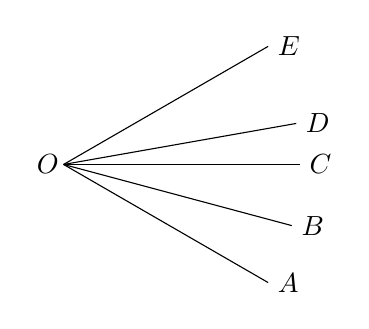
\begin{tikzpicture}[>=latex, scale=1]
\foreach \x/\xtext in {30/E, 10/D, 0/C, -15/B, -30/A}
{
	\draw(0,0)--(\x:3)node[right]{$\xtext$};
}
\node at (-.2,0){$O$};
    \end{tikzpicture}
    \caption*{第7题}
    \end{minipage}
    \begin{minipage}[t]{0.48\textwidth}
    \centering
    \begin{tikzpicture}[>=latex, scale=1]
\tkzDefPoints{0/0/O, 3/0/A, 1.5/0/P, 1/1/Q, 2/2/B}
\tkzLabelPoints[below](O,P,A)
\tkzLabelPoints[above](Q,B)
\tkzDrawSegments(O,B O,A)
\tkzDrawPoints(Q,P)
    \end{tikzpicture}
    \caption*{第8题}
    \end{minipage}
    \end{figure}




\subsection{角度和旋转}
在前面我们说明了可以用以$A$点为端点的一条射线来
表示一个由$A$点出发的方向。设射线$AB$和$AC$分别表示一个
由$A$点出发的两个方向,那么这两条射线所成的角也可以看
作是一条以$A$点为端点的射线,从$AB$的位置沿着平面旋转
到$AC$的位置而成的图形。象度量线段$\overline{PQ}$的长度就是度量表
示$P$、$Q$这两个位置之间的距离一样;度量射线$AB$和$AC$所
表示的这两个方向之间的差别也就是度量这两条射线之间所
夹的“角度”。而角度也就可以看成是旋转量了。下面采用旋
转的观点对于角度的度量再作一初步的探讨:

\subsubsection{角度的大小}
\begin{figure}[htp]
	\centering
\begin{tikzpicture}[>=latex]
\begin{scope}
\tkzDefPoint(2,0){B}	
\tkzDefPoint(20:2){B'}
\tkzDefPoint(45:2){C}
\tkzDefPoint(100:1.8){C'}
\tkzDefPoint(0,0){A}
\tkzDrawPoints(B,C,B',C')
\tkzLabelPoints[left](A,C',C)
\node at (0,0)[below]{$A'$};
\tkzLabelPoints[below](B',B)
\tkzDrawLines[add=0 and .5, ->](A,B A,B' A,C A,C')
\end{scope}
\begin{scope}[xshift=5cm]
\draw (0,0) rectangle (4,3);
\tkzDefPoints{.5/1.5/A', 3/2.5/C', 3/.5/B'}
\tkzDrawPoints(A',B',C')
\tkzLabelPoints[below](A',C',B')
\tkzDrawLines[add=0 and .2 ](A',B' A',C')
\end{scope}
\end{tikzpicture}
	\caption{}
\end{figure}

如图1.29所示,$\angle BAC$和$\angle B'A'C'$分别是以$A$和$A'$为
顶点的两个角,用一张透明的塑胶片,先把它盖在$\angle B'A'C'$
的上面,用笔把$\angle B'A'C'$复印到塑胶片上。然后把塑
胶片移到$\angle BAC$的上面,调整其位置使得顶点$A$和顶点$A'$
相重合;再用一个针插在$A$、$A'$点之上,这样,塑胶片仍然
可以绕着针尖所插的$A'$点旋转,但是$A$、$A'$点依然确保重
合。适当旋转可以使得两个角的边$AB$和$A'B'$重合,而且
“角区”位于相重边的同侧(图1.30)。
\begin{figure}[htp]\centering
    \begin{minipage}[t]{0.48\textwidth}
    \centering
\begin{tikzpicture}[>=latex, scale=1]
    \tkzDefPoints{0/0/A, 2/0/B', 3/0/B}
	\tkzDefPoint(40:2.5){C}
	\tkzDefPoint(60:2.5){C'}
\tkzLabelPoints[below](A,B',B)
\tkzLabelPoints[above](C,C')
\tkzDrawLines[add=0 and .4 ](A,B A,C' A,C)
\tkzDrawPoints(A,B',C',C)
\node at (0,0)[left]{$A'$};
    \end{tikzpicture}
    \caption{}
    \end{minipage}
    \begin{minipage}[t]{0.48\textwidth}
    \centering
    \begin{tikzpicture}[>=latex, scale=1]
		\tkzDefPoints{0/0/A, 3/0/B}
		\tkzDefPoint(40:3){C}
		\tkzDefPoint(100:2.5){D}	
		\tkzDrawLines[add=0 and .3 ](A,B A,C A,D)	
		\tkzLabelPoints[below](A,C,B)
		\tkzLabelPoints[left](D)
		\tkzDrawPoints(A,B,C,D)
		\tkzMarkAngles[mark=none,->, size=.6](B,A,C C,A,D)
		\tkzMarkAngles[mark=none,->, size=.8](B,A,D)
    \end{tikzpicture}
    \caption{}
    \end{minipage}
    \end{figure}


这样,两角之间有下列三种可能的位置关系:
\begin{itemize}
	\item 它们的另一边也重合,那么就说这两个角相等,记作
	$\angle B'A'C'=\angle BAC$;
	\item $A'C'$落在$\angle BAC$的内部,那么就说$\angle B'A'C'$小于$\angle BAC$, 记作$\angle B'A'C'<\angle BAC$;
	\item $A'C'$落在$\angle BAC$的外部,那么就说$\angle B'A'C'$大于$\angle BAC$, 记作$\angle B'A'C'>\angle BAC$。
\end{itemize}

\subsubsection{两角的相加}
如图1.31所示,$\angle BAC$和$\angle CAD$两个角的顶点相同,
有一条边相重合(即射线$AC$),而且两者的角区分居于公共
边的两侧,就说$\angle BAD$为$\angle BAC$和$\angle CAD$之和,即$\angle BAD=\angle BAC+\angle CAD$. 这时由等式的性质,又可知$\angle BAC=\angle BAD-\angle CAD$,$\angle CAD=\angle BAD-\angle BAC$。


当两个角相加后是一个平角时,就说这两个角\textbf{互为补角},
其中一个角叫做另一个角的补角。简称为\textbf{互补}(图1.32(1))。
一个角如果和它的补角相等,这个角叫做\textbf{直角}(图1.32(2))。

\begin{figure}[htp]
	\centering
\begin{tikzpicture}
\begin{scope}
\tkzDefPoints{-2/0/A, 0/0/O, 2/0/B, -1.5/1.5/C}
\tkzDrawSegments(A,B  C,O)
\tkzMarkAngles[mark=none, size=.6](C,O,A)
\tkzMarkAngles[mark=none, size=.4](B,O,C)
\tkzLabelAngle[pos=.8](C,O,A){$\alpha$}
\tkzLabelAngle[pos=.6](B,O,C){$\beta$}
\node at (0,-.5){(1)};
\end{scope}
\begin{scope}[xshift=5cm]
	\tkzDefPoints{-2/0/A, 0/0/O, 2/0/B, 0/2/C}
	\tkzDrawSegments(A,B  C,O)
	\tkzMarkRightAngle[size=.3](C,O,A)
	\tkzMarkRightAngle[size=.2](B,O,C)
	\node at (0,-.5){(2)};
\end{scope}
\end{tikzpicture}
	\caption{}
\end{figure}

小于直角的角叫做\textbf{锐角},大于直角小于平角的角叫做\textbf{钝
角}。如图1.33所示,$\angle AOB$为锐角,$\angle CPD$为钝角。
\begin{figure}[htp]
	\centering
\begin{tikzpicture}[>=latex]
\begin{scope}
\tkzDefPoints{3/0/A, 0/0/O, 1.8/1.8/B, 0/2/C}
\tkzDrawSegments(A,O B,O)
\tkzDrawSegments[dashed](C,O)
\tkzMarkAngles[mark=none, size=.6,->](A,O,B)
\tkzLabelPoints[below](A,O,B)
\node at (1.5,-.75){(1)};
\end{scope}
\begin{scope}[xshift=7cm]
	\tkzDefPoints{-2/0/A, 0/0/P, 2/0/C, -1.8/1.8/D, 0/2/E}
	\tkzDrawSegments[dashed](A,P P,E)
	\tkzDrawSegments(C,P P,D)
	\tkzMarkAngles[mark=none, size=.4,->](C,P,D)
	\tkzLabelPoints[below](C,P,D)
	\node at (0,-.75){(2)};
\end{scope}
\end{tikzpicture}
	\caption{}
\end{figure}

如果两个角相加的和等于直角,这两角叫做互为余角。
其中一个角叫做另一个角的余角。例如图1.34中的$\angle\alpha+\angle\beta=$直角,则$\angle\alpha$、$\angle\beta$互为余角。

\begin{figure}[htp]
	\centering
\begin{tikzpicture}[>=latex]
\begin{scope}
\tkzDefPoints{2/0/A, 0/0/O}
\tkzDefPoint(30:1.8){B1}
\tkzDrawSegments(A,O B1,O)
\tkzMarkAngles[mark=none, size=.6](A,O,B1)
\tkzLabelAngle[pos=.8](A,O,B1){$\alpha$}
\end{scope}
\begin{scope}[xshift=4cm]
	\tkzDefPoints{2/0/A, 0/0/O}
\tkzDefPoint(60:1.8){B2}
\tkzDrawSegments(A,O B2,O)
\tkzMarkAngles[mark=none, size=.6](A,O,B2)
\tkzLabelAngle[pos=.8](A,O,B2){$\beta$}
\end{scope}
\begin{scope}[xshift=8cm]
	\tkzDefPoints{2/0/A, 0/0/O, 0/2/C}
\tkzDefPoint(30:1.8){B1}
\tkzDrawSegments(A,O B1,O O,C)
\tkzMarkAngles[mark=none, size=.6](A,O,B1)
\tkzLabelAngle[pos=.8](A,O,B1){$\alpha$}
\tkzMarkAngles[mark=none, size=.5](B1,O,C)
\tkzLabelAngle[pos=.8](B1,O,C){$\beta$}
\end{scope}
\end{tikzpicture}
	\caption{}
\end{figure}

\subsubsection{角的度量与量角器}
角的度量和线段的度量的做法基本上是相同的。也是先
取定一个角度单位,然后用这个单位,或把它适当等分所得
的分单位去和一个要量的角来比较大小。常用的单位是把一
个平角分成180等份,其中一份叫做1度;再把1度分成60
等份,其中一份叫做1分;再把1分分成60等份,其中一份叫
做1秒。常用的符号是在数字的右上角上标以“${}^{\circ}$”表示
度,“$'$”表示分,
“$''$”表示秒。例如:35度12分30秒就
写成$35^{\circ}12'30''$。

平角$=180^{\circ}$, 平角的二等分角(即平角的一半)就是直
角,直角$=90^{\circ}$. 四个直角相加得一周角,周角$=360^{\circ}$.

\begin{figure}[htp]
	\centering
	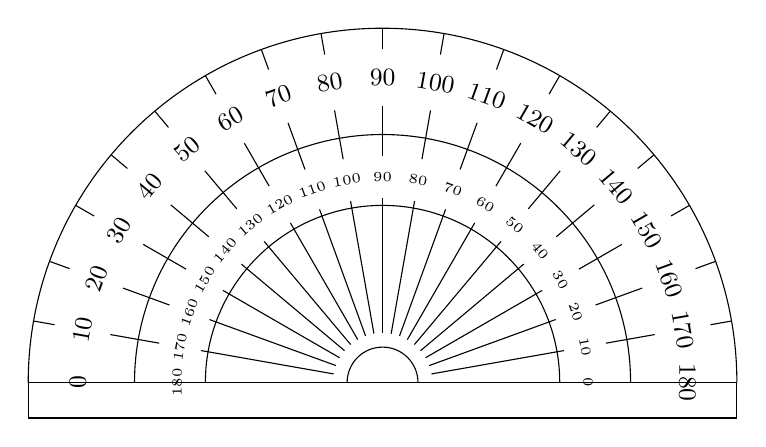
\begin{tikzpicture}[scale=.9]
\draw(-5,0) rectangle (5,-.5);	
\foreach \x in {.5, 2.5,3.5,5}
{
	\draw(\x ,0) arc (0:180:\x );
}
\foreach \x in {0, 10,20,...,170,180}
{
	\draw (\x:0.7)--(\x:2.6);
	\draw (\x:3.2)--(\x:3.9);
	\draw (\x:4.7)--(\x:5);
	\node[rotate=-90+\x] at (\x:2.9){\tiny \x};
	\node[rotate=90-\x] at (180-\x:4.3){\small \x};
}
\end{tikzpicture}
	\caption{}
\end{figure}


度量长度的常用工具是刻有等分刻度的直尺,相应地度
量角度的常用工具是图1.35所示的量角器。量角器是一个
具有180个等分刻度的半圆形塑胶板,当我们要去量一个给
定的角的角度时,先把顶点和这个半圆板的圆心叠合,然后
使得直径和角的一边相重合;那么角的另一边通过半圆的位
置的刻度就是所量角度的近似值。如图1.36中的$\angle BAC$,
$AB$与$0^{\circ}$线重合,$AC$恰好落在$40^{\circ}$的刻度上,所以$\angle BAC=40^{\circ}$.

\begin{figure}[htp]
	\centering
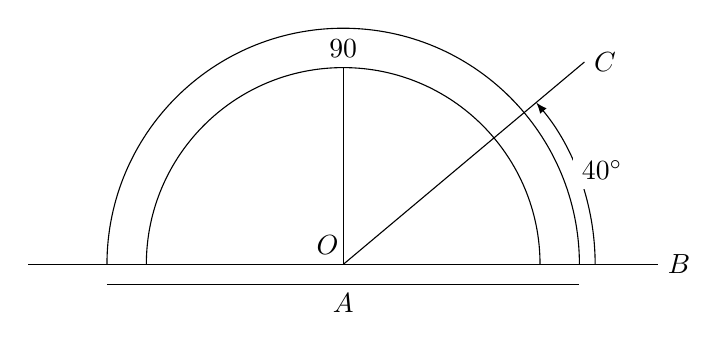
\begin{tikzpicture}[>=latex]
\draw (-4,0)--(4,0)node[right]{$B$};
\draw (2.5,0) arc (0:180:2.5);
\draw (3,0) arc (0:180:3);
\draw(0,0) --(40:4)node[right]{$C$};
\node at (-.2,0)[above]{$O$};
\draw(0,0)--(0,2.5)node[above]{$90$};
\draw[->](3.2,0) arc(0:40:3.2);
\node at (20:3.5)[fill=white]{$40^{\circ}$};
\draw(-3,-.25)--node[below]{$A$}(3,-.25);

\end{tikzpicture}	
	\caption{}
\end{figure}

\begin{example}
	求$30^{\circ}19'21''$与$18^{\circ}40'42''$的和。
\end{example}

\begin{solution}
\[30^{\circ}19'21''+18^{\circ}40'42''=48^{\circ}59'63''=49^{\circ}3''\]
\end{solution}

\begin{example}
	把$3.62^{\circ}$化成度、分、秒。
\end{example}

\begin{solution}
$\because\quad 1^{\circ}=60',\qquad \therefore\quad 0.62^{\circ}=60'\x 0.62=37.2'$

$\because\quad 1'=60'',\qquad \therefore\quad 0.2'=60''\x 0.2=12''$

$\therefore\quad 3.62^{\circ}=3^{\circ}37'12''$
\end{solution}

\begin{example}
	把$15^{\circ}18'15''$化为度。
\end{example}


\begin{solution}
	先把$15''$化为分:
\[\frac{15''}{60''}=0.25'\]
$\therefore\quad 18'15''=18.25'$。
再把$18.25'$化为度:
\[\frac{18.25'}{60'}\approx 0.304^{\circ}\]
$\therefore\quad 15^{\circ}18'15''\approx 15.304^{\circ}$.
\end{solution}

\subsubsection{对顶角相等和两条直线互相垂直}

如图1.37所示 直线$AB$和$CD$相交于$O$点,这时,
$\angle AOC$和$\angle BOD$中$OA$和$OB$, $OC$和$OD$都互为反向延长
线。象这样,一个角的两边分别是另一个角的两边的反向延
长线时,我们就称这两个角为\textbf{对顶
角}。

如果两个角是对顶角,那么它
们之间有什么关系呢?由图1.37
可知,$\angle AOC$和$\angle AOD$互为补
角,即$\angle AOC+\angle AOD=180^{\circ}$;
$\angle BOD$和$\angle AOD$也互为补角,即$\angle BOD+\angle AOD=180^{\circ}$,
因而$\angle AOC+\angle AOD=\angle BOD+\angle AOD$, 所以,$\angle AOC=\angle BOD$.

总结上述事实就成为下述性质:
\textbf{对顶角相等}

\begin{example}
	如果两条直线$AB$、$CD$相交于$O$点(图1.37),
$\angle AOC=40^{\circ}$, 求$\angle BOD$, $\angle AOD$, $\angle COB$的度数。
\end{example}

\begin{figure}[htp]
	\centering
\begin{tikzpicture}
\tkzDefPoints{-2/.75/A, 2/-.75/B, -2/-.75/C, 2/.75/D,0/0/O}
\tkzLabelPoints[above](A,B,C,D,O)
\draw(A)--(B);
\draw(C)--(D);
\tkzMarkAngles[mark=none, size=.5](A,O,C B,O,D)
\end{tikzpicture}
	\caption{}
\end{figure}

\begin{solution}
	两条直线$AB$、$CD$相交于$O$点

$\therefore\quad \angle AOC$和$\angle BOD$是对顶角,
$\therefore\quad \angle AOC=\angle BOD$(对顶角相等)。

$\because\quad \angle AOC=40^{\circ}$

$\therefore\quad \angle BOD=40^{\circ}$.

又:$\angle AOC+\angle AOD=180^{\circ}$,

$\therefore\quad \angle AOD=180^{\circ}-\angle AOC=180^{\circ}-40^{\circ}=140^{\circ}$.

$\because\quad \angle AOD=\angle COB$(对顶角相等)

$\therefore\quad \angle COB=140^{\circ}$
\end{solution}


由于两条直线相交得出四个角,根据对顶角的概念可
知,这四个角分为两双对顶角,当然每双对顶角都是相等
的。并且不难看出,如果两条直线相交得出的四个角中,有
一个是直角,那么其余的三个角也都是直角。

当两条直线相交成直角时,这两条直线就叫做\textbf{互相垂直}。其中一条叫做另一条的垂线,交
点叫做垂足。如图1.38所示$\ell_1$和$\ell_2$
互相垂直,$O$是它们的垂足,记作
$\ell_1\bot \ell_2$于$O$点。符号“$\bot$”读作“垂直
于”。

因为三角板中有一个角是直角,
所以可以用三角板来画垂线。






\begin{example}
	
\end{example}

\begin{solution}
	
\end{solution}


\begin{example}
	
\end{example}

\begin{solution}
    
\end{solution}


\begin{example}
	
\end{example}

\begin{solution}
    
\end{solution}

\begin{example}
	
\end{example}


\begin{solution}
    
\end{solution}


\begin{example}
    
\end{example}

\begin{solution}
    
\end{solution}


\begin{example}
    
\end{example}
\begin{solution}
    
\end{solution}


\begin{example}
    
\end{example}


\begin{solution}
    
\end{solution}





\begin{blk}
	
\end{blk}

\begin{blk}
	
\end{blk}

\begin{blk}
	
\end{blk}

\begin{blk}
	
\end{blk}




\begin{example}
	
\end{example}

\begin{solution}
	
\end{solution}


\begin{example}
	
\end{example}

\begin{solution}
    
\end{solution}


\begin{example}
	
\end{example}

\begin{solution}
    
\end{solution}

\begin{example}
	
\end{example}


\begin{solution}
    
\end{solution}


\begin{example}
    
\end{example}

\begin{solution}
    
\end{solution}


\begin{example}
    
\end{example}
\begin{solution}
    
\end{solution}


\begin{example}
    
\end{example}


\begin{solution}
    
\end{solution}

\begin{ex}
\begin{enumerate}
	\item 已知线段$a,b$, 求作一线段等于$a+b$; $a-b\; (a>b)$.
	\item 任意画一个$\triangle ABC$, 利用它的三边之长再画一个三角形
$A'B'C'$, 使得$\triangle A'B'C'\cong \triangle ABC$.
	\item 先任意画一个$\angle \alpha$, 再画一个$\angle \beta$, 使得$\angle \beta=\angle\alpha$.
	\item 任意
	画一个$\angle ABC$, 试作$\angle ABC$的平分线。
	\item 已
	知$\angle \alpha$ (小于$180^{\circ}$), 和两条线段$m,n$, 求作一个
	$\triangle 
	ABC$, 使得$\angle A=\angle \alpha$, $\overline{AB}=m$, $\overline{AC}=n$.
	\item 已知$\overline{AB}$, 作$\overline{AB}$的垂直平分线。
	\item 已知$\triangle ABC$, 过$A,B,C$分别作$\overline{BC}$, $\overline{AC}$, $\overline{AB}$所在的
	直线的垂线。
	\item 画一个平角$\angle AOB$, 再将$\angle AOB$二等分,四等分。
	\item 将$\overline{AB}$四等分。
	\item 过$\triangle ABC$各顶点分别作对边的平行线。
\end{enumerate}
\end{ex}

\begin{figure}[htp]
	\centering
\begin{tikzpicture}
\tkzDefPoints{0/0/B, 2/0/C, 3.5/2.5/A}
\tkzDrawLines(A,C A,B)
\tkzDrawLines[add=.5 and 1](B,C)
\tkzLabelPoints[below](B,C)
\tkzLabelPoints[right](A)
\end{tikzpicture}
	\caption*{第7题}
\end{figure}

\subsection*{习题1.5}
\begin{enumerate}
	\item 作一个角等于:$\angle\alpha+\angle \beta$;$\angle\alpha-\angle \beta$.
\begin{figure}[htp]
	\centering
\begin{tikzpicture}
\tkzDefPoints{0/0/A, 2/0/B, 1.5/1.2/C}
\tkzDrawSegments(A,B A,C)
\tkzDefPoints{4/0/A', 5.5/0/B', 5.5/1.3/C'}
\tkzDrawSegments(A',B' A',C')

\tkzMarkAngles[mark=none, size=.4](B,A,C B',A',C')
\tkzLabelAngle[pos=.6](B,A,C){$\alpha$}
\tkzLabelAngle[pos=.6](B',A',C'){$\beta$}
\end{tikzpicture}
	\caption*{第1题}
\end{figure}
	\item 作一个三角形,使其两个角分别等于$\angle\alpha$、$\angle \beta$, $\angle \alpha$
	的对边等于已知线段$a$.
	\begin{figure}[htp]
	\centering
\begin{tikzpicture}
	\tkzDefPoints{0/0/A, 2/0/B, 1.5/1.2/C}
	\tkzDrawSegments(A,B A,C)
	\tkzDefPoints{4/0/A', 5.5/0/B', 5.5/1.3/C'}
	\tkzDrawSegments(A',B' A',C')
	
	\tkzMarkAngles[mark=none, size=.4](B,A,C B',A',C')
	\tkzLabelAngle[pos=.6](B,A,C){$\alpha$}
	\tkzLabelAngle[pos=.6](B',A',C'){$\beta$}

	\draw(0,2)--node[above]{$a$}(2.5,2);
\end{tikzpicture}
	\caption*{第2题}
\end{figure}

	(提示:先设法作出要作的三角形的第三个角,然后再
	利用基本作图题4的方法作图)

	\item 作一个三角形的各边的垂直平分线,看是否相交于一点。
	\item 作一个三角形的三个内角的平分线,看是否交于一点。
	\item $P$是$\triangle ABC$内一点,过$P$作三边的垂线。
	\item 试作下列花纹图形:
\begin{figure}[htp]
	\centering
\begin{tikzpicture}[scale=.7]
\begin{scope}
\draw(0,0) rectangle (2,2);
\draw(2,0) rectangle (4,2);
\draw(4,0) rectangle (6,2);

\foreach \x in {0,2,4}
{
	\draw(\x+1,0)--(\x+1,2);
	\draw(\x,0) arc (-90:90:1);
	\draw(\x,0) arc (180:0:1);
	\draw(\x,2) arc (90:-90:1);
	\draw(\x,2) arc (180:360:1);
    \draw(\x+2,0) arc (270:90:1);
}
\draw(0,1)--(6,1);

\end{scope}

\begin{scope}[xshift=10cm]
\tkzDefPoints{0/0/A, 2/0/B,1/1.732/C}
\foreach \x in {A,B,C}
{
	\draw(\x) circle (1);
}
\tkzDrawPolygon[fill=white](A,B,C)
\end{scope}
\begin{scope}[xshift=2cm, yshift=-3cm]
	\draw(0,0)circle(2);
\draw(30:2) arc (90:210:2);
\draw(30:2) arc (-30:-150:2);
\draw(-30:2) arc (-90:-210:2);
\draw(-30:2) arc (30:150:2);
\draw(90:2) arc (30:-90:2);
\draw(-90:2) arc (-30:90:2);

\end{scope}

\begin{scope}[xshift=6cm, yshift=-3cm]
\draw(2,0)circle(2);
\foreach \x in {1,2,3}
{
	\draw(0,0) arc (180:0:\x/2);
	\draw(4,0) arc (0:-180:\x/2);
}
\draw(0,0)--(4,0);
\end{scope}

\begin{scope}[xshift=14cm, yshift=-3cm]
	\draw(0,0)circle(2);
\draw(-2,0)--(2,0);
\draw(0,-2)--(0,2);
\foreach \x in {0,2}
{
	\draw(\x-2,0) arc (-180:0:.5);
	\draw(\x-1,0) arc (180:0:.5);
	\draw(0,\x) arc (90:270:.5);
	\draw(0,\x-1) arc (90:-90:.5);
}
\end{scope}
\end{tikzpicture}
	\caption*{第6题}
\end{figure}
\end{enumerate}

\section*{小结}

在这一章实验几何中,我们对于常见、常用的空间的某
些基本概念如位置、通路、方向、全等、相似等作了分析,
从而确立了一系列的几何概念如点、直线、平面;射线、
角、平行;长度、角度、全等形、相似形等等。我们还通过
观察与实验,分析与归纳,从而总结出空间的一些性质如
“两点确定一条直线”、“不共线三点确定一个平面”等
等,这些都是以后进一步研究几何学的基础,为了便于以后
查看,我们把本章所述的几何概念和性质列举如下\footnote{基本作图题就不再列出了。}:

\subsection*{点、直线、平面及其相互关系}

\begin{blk}
	{概念} 点是位置的反映;线是通路的反映;线段是两点
间的最短通路;直线是线段向两端无限延伸而得到的图形。
\end{blk}

\begin{blk}
	{性质}
\begin{enumerate}
	\item 两点确定一条直线。
	\item 当一个平面包含两个点$A$、$B$时,它也就包含整条直线$AB$.
	\item 空间不共线三点确定一个平面。
	\item 两个相交平面的交线是一条直线,对于空间一条
	给定的直线,存在着无数个包含这条直线的平面。
\end{enumerate}
\end{blk}

\subsection*{射线、角、平行与三角形}

\begin{blk}
	{概念} 直线上一点一旁的部分叫做射线。一条以点$A$为
端点的射线表示由$A$点出发的一个方向;以同一点为端点的
两条射线所组成的图形叫做角,它体现了这两条射线所表示
的两个方向之间的差别;同一平面上的两条直线被一条直线
所截,如果同位角相等,就称这两条直线互相平行;两个形
状和大小完全相同的图形叫做全等形,两个平面图形全等的
实践检验方法就是它们完全重合;两个形状相同大小不一定
相同的图形叫做相似形;两个多边形相似的条件是它们的角
对应相等,对应边成比例。
\end{blk}

\begin{blk}{性质}
\begin{enumerate}
	\item 两条线段全等的唯一条件就是它们的长度相
	等。
	\item 两个角全等的唯一条件就是它们的角度相等。
	再者,在平面内给定一条射线$AB$和$\angle \alpha$, 在直线$AB$两侧
	分别存在着唯一的一条射线$AC$和$AC'$, 使得$\angle BAC=
	\angle BAC'=\angle\alpha$
	\item 三角形的三个内角和是一个平角。
	\item 过直线$\ell$外一点$P$只有一条直线和$\ell$平行。
	\item 在同一平面内,过已知点作已知直线的垂线只
	有一条。
	\item 两个三角形如果有两边一夹角分别对应相等,
	它们就全等(SAS).
	\item 两个三角形如果有两角一夹边分别对应相等,
	它们就全等(ASA).
	\item 两个三角形如果三条边分别对应相等,它们就
	全等(SSS).
	\item 两个三角形如果有两个角对应相等,它们就相
	似。
	\end{enumerate}
\end{blk}

\section*{复习题一}
\begin{enumerate}
	\item $A$、$B$、$C$、$D$是依此顺序位于一条直线上的四个点,并
且$\overline{AB}=\overline{BD}$, $\overline{BC}=\overline{CD}$, 把下列各组线段的长度关系,
分别用式子表示:
\begin{multicols}{3}
\begin{enumerate}
	\item $\overline{AB}$和$\overline{BC}$
	\item $\overline{AB}$和$\overline{AD}$
	\item $\overline{AD}$和$\overline{CD}$
\end{enumerate}
\end{multicols}

\item 射线$AB$和射线$BA$所表示的方向是否相同?
\item 两点间的距离是什么?一点到一条直线的距离是什么?
\item 在四边形$ABCD$内找一点$P$, 使得$P$点到$A$、$B$、$C$、$D$
四顶点的距离之和最短?你猜想这一点在什么位置?并用
线是两点间的最短通路来说明你的猜想?
\item 在$\triangle ABC$中,如果$\overline{AB}=\overline{AC}$, 并且$P_1$、$P_2$是$\overline{BC}$上任
意两点,那么:
\begin{enumerate}
\item 量出$P_1$点到$\overline{AB}$、$\overline{AC}$两边的距离之和;
\item 量出$P_2$点到$\overline{AB}$、$\overline{AC}$两边的距离之和;
\item 比较一下(a)与(b)所得的结果,你能作出什么
猜想?
\end{enumerate}

\begin{figure}[htp]\centering
	\begin{minipage}[t]{0.48\textwidth}
	\centering
  \begin{tikzpicture}[>=latex, scale=1]
\tkzDefPoints{0/0/B, 2.5/-.2/C, 3/1/D, 2/1.5/A}
\tkzDrawPolygon(A,B,C,D)
\tkzLabelPoints[below](B,C)
\tkzLabelPoints[right](D)
\tkzLabelPoints[above](A)   
	\end{tikzpicture}
	\caption*{第4题}
	\end{minipage}
	\begin{minipage}[t]{0.48\textwidth}
	\centering
	\begin{tikzpicture}[>=latex, scale=1]
\tkzDefPoints{0/0/B, 3/0/C, 1.5/2/A, .7/0/P_1, 1.7/0/P_2}
\tkzDrawPolygon(A,B,C)
\tkzLabelPoints[below](B,C,P_1,P_2)
\tkzLabelPoints[above](A)   
\tkzDrawPoints(P_1,P_2)

	\end{tikzpicture}
	\caption*{第5题}
	\end{minipage}
	\end{figure}

\item 在一个平面上三条直线的位置关系有几种情况?
\item 长24cm的线段,被分成不相等的四部分,首尾两部分
的中点间的距离是20cm, 求中间两部分中点间的距离是多
少厘米?
\item 如果时针和分针组成$7^{\circ}30'$的角,而分针指着
\begin{multicols}{2}
	\begin{enumerate}
		\item 3;
		\item 9
	\end{enumerate}
\end{multicols}
那么现在是几点钟?
\item 两个角度数的比为7:3, 差为$72^{\circ}$, 这两个角是否互为
补角?
\item 如图,已知$\angle ABC$和$\angle CBD$互为补角,$EB\bot AB$, $\angle ABC=92^{\circ}$, $BF$是$\angle CBD$的平分线,求$\angle EBF$是多少
度?
\item 已知$\angle AOB$被$OC$分成两部分,这两部分的差是$30^{\circ}$, 
$\angle AOB$的平分线是$OM$, 求$\angle COM$的度数。
\item 五个点$A$、$B$、$C$、$D$、$E$排列在一条直线上,而且$D$点
在$A$点右边4m的地方,$C$点在$E$点右边5m的地方,又$B$
点在$E$点左边5m的地方,$B$点在$A$点左边4m的地方,
问:
\begin{enumerate}
	\item 正好在中间的是那个点?
	\item $D$点在$E$点右边
多少米远的地方?
\end{enumerate}

\begin{figure}[htp]\centering
	\begin{minipage}[t]{0.48\textwidth}
	\centering
  \begin{tikzpicture}[>=latex, scale=1]
\tkzDefPoints{-1/0/A, 0/0/B, 3/0/D, 0/3/E}
\tkzDefPoint(88:3){C}
\tkzDrawLine[bisector](C,B,D)  \tkzGetPoint{F'}
\tkzDefPointWith[linear, K=2](B,F')  \tkzGetPoint{F}
\tkzDrawSegments(A,D B,E B,C B,F)
\tkzLabelPoints[below](A,B,D)
\tkzLabelPoints[right](C,F)
\tkzLabelPoints[left](E)
	\end{tikzpicture}
	\caption*{第10题}
	\end{minipage}
	\begin{minipage}[t]{0.48\textwidth}
	\centering
	\begin{tikzpicture}[>=latex, scale=1]
		\tkzDefPoints{-2/0/A, 0/0/O, 2/0/B}
\tkzDefPoint(70:2.5){C}
\tkzDrawLine[bisector](C,O,B)  \tkzGetPoint{E'}
\tkzDrawLine[bisector](A,O,C)  \tkzGetPoint{D'}
\tkzDefPointWith[linear, K=1.56](O,E')  \tkzGetPoint{E}\tkzDefPointWith[linear, K=2](O,D')  \tkzGetPoint{D}
\tkzLabelPoints[below](A,B,O)
\tkzLabelPoints[right](C,E)
\tkzLabelPoints[left](D)
\tkzDrawSegments(A,B D,O C,O E,O)
	\end{tikzpicture}
	\caption*{第13题}
	\end{minipage}
	\end{figure}

\item 已知$\angle AOC$和$\angle COB$互为补角,$OD$、$OE$分别是
$\angle AOC$和$\angle COB$的平分线,那么
\begin{enumerate}
	\item $OD$是否垂直$OE$?为什么?
	\item $\angle AOD$与$\angle BOE$是否互余?为什么?
\end{enumerate}

\item 在已知$\triangle ABC$中,$\angle B=\angle C$, $\angle A=4\angle B$, 问$\angle A$, $\angle B$、$\angle C$各等于多少度?
\item 已知$\triangle ABC$中,$\angle A:\angle B:\angle C=1:2:3$, 求$\angle A$、
$\angle B$、$\angle C$各等于多少度?
\item 在$\triangle ABC$中,$\angle A=60^{\circ}$, $\angle B=\angle C$, 如果$\angle B$、$\angle C$
的平分线相交于$O$点,问$\angle BOC$等于多少度?
\item 已知如图,在$\triangle ABC$中,
$\overline{BA}\bot \overline{AC}$, $\overline{AD}\bot \overline{BC}$, $\angle BAD=30^{\circ}$, 求$\angle x$, $\angle y$, $\angle z$的
度数?
\begin{figure}[htp]
	\centering
\begin{tikzpicture}[scale=1.4]
	\tkzDefPoints{0/0/B, 4/0/C, 1/1.732/A, 1/0/D}
\tkzDrawPolygon(A,B,C)
\tkzDrawSegments(A,D)
\tkzMarkRightAngle[size=.15](A,D,C)
\tkzLabelPoints[below](B,C,D)
\tkzLabelPoints[above](A)
\tkzMarkAngles[mark=none, size=.3](C,B,A B,A,D A,C,B)
\tkzMarkAngles[mark=none, size=.25](D,A,C)
\tkzLabelAngle[pos=.4](C,B,A){$y$}
\tkzLabelAngle[pos=.6](B,A,D){$30^{\circ}$}
\tkzLabelAngle[pos=.4](A,C,B){$z$}
\tkzLabelAngle[pos=.4](D,A,C){$x$}

\end{tikzpicture}
	\caption*{第17题}
\end{figure}

\item 求图中$\angle\alpha$, $\angle\beta$的大小。

\begin{figure}[htp]
	\centering
\begin{tikzpicture}
\begin{scope}
\tkzDefPoints{0/0/A, 2/0/B, -1/0/A', 4/0/B'}
\tkzDefPoint(70:4){C}
\tkzDrawSegments(A,C B,C)
\tkzDrawLines[add=.5 and .5](A,B)
\tkzMarkAngles[mark=none, size=.3](C,A,A' B',B,C)
\tkzMarkAngles[mark=none, size=.4](A,C,B)
\tkzLabelAngle[pos=.6](C,A,A'){$110^{\circ}$}
\tkzLabelAngle[pos=.6](B',B,C){$100^{\circ}$}
\tkzLabelAngle[pos=.6](A,C,B){$\alpha$}
\end{scope}
\begin{scope}[xshift=5cm]
\tkzDefPoints{0/0/B, 3/0/C, 1.2/2.6/A, 2.7/1/D, -1/0/B', 4/0/C'}
\tkzDrawPolygon(A,B,C,D)
\tkzDrawLines[add=.25 and .25](C,B)
\tkzLabelPoints[below](B,C)
\tkzLabelPoints[above](A)
\tkzLabelPoints[right](D)
\tkzMarkAngles[mark=none, size=.3](A,B,B' C',C,D A,D,C B,A,D)
\tkzLabelAngle[pos=.6](A,B,B'){$120^{\circ}$}
\tkzLabelAngle[pos=.6](C',C,D){$100^{\circ}$}
\tkzLabelAngle[pos=.6](A,D,C){$\beta$}
\tkzLabelAngle[pos=.6](B,A,D){$88^{\circ}$}


\end{scope}
\end{tikzpicture}
	\caption*{第18题}
\end{figure}

\item 已知$\triangle ABC$中,$\angle ABC=90^{\circ}$, 当$A$点和$B$点相重合
折叠时,设折痕为$\overline{DE}$, 那么$\angle EBC=\angle C$, 为什么?
\item 已知如图,直线$EF$, $GH$和直线$MN$相交于$A,B$, $AC$
平分$\angle MAF$, $BD$平分$\angle ABH$, 并且$\angle MAF=\angle ABH$, 问:
\begin{enumerate}
	\item $EF$与$GH$是否平行?为什么?
	\item $AC$与$BD$是否平行?为什么?
\end{enumerate}

\begin{figure}[htp]\centering
	\begin{minipage}[t]{0.48\textwidth}
	\centering
  \begin{tikzpicture}[>=latex, scale=1]
\tkzDefPoints{0/0/B, 3/0/C, 0/4/A}
\tkzDefMidPoint(A,B)\tkzGetPoint{D}
\tkzDefMidPoint(A,C)\tkzGetPoint{E}
\tkzDrawPolygon(A,B,C)
\tkzDrawPolygon[pattern=north east lines](B,D,E)
\tkzLabelPoints[right](E)
\tkzLabelPoints[left](D)
\tkzLabelPoints[below](B,C)
\tkzLabelPoints[above](A)

	\end{tikzpicture}
	\caption*{第19题}
	\end{minipage}
	\begin{minipage}[t]{0.48\textwidth}
	\centering
	\begin{tikzpicture}[>=latex, scale=1]
\tkzDefPoints{-1/1/G, 3/1/H, -1/2.5/E, 3/2.5/F, -.5/0/N, 2/4/M}
\tkzDrawSegments(E,F G,H M,N)
\tkzInterLL(E,F)(M,N)  \tkzGetPoint{A}
\tkzInterLL(G,H)(M,N)  \tkzGetPoint{B}
\tkzLabelPoints[left](E,G)
\tkzLabelPoints[right](F,H)
\tkzLabelPoints[above left](A,B)
\tkzLabelPoints[above](M)
\tkzLabelPoints[below](N)
\tkzDefLine[bisector, normed](M,A,F) \tkzGetPoint{C'}
\tkzDefLine[bisector, normed](M,B,H) \tkzGetPoint{D'}
\tkzDefPointWith[linear,K=2](A,C')\tkzGetPoint{C}
\tkzDefPointWith[linear,K=2](B,D')\tkzGetPoint{D}
\tkzDrawSegments(A,C B,D)
\tkzLabelPoints[right](C,D)
	\end{tikzpicture}
	\caption*{第20题}
	\end{minipage}
	\end{figure}

	\item 已知如图,并且$\angle 1=\angle 2$, 那么$\ell$是否平行$m$?为什
么?
\item 已知:
\begin{enumerate}
	\item $\overline{AB}=5$cm, $\overline{AC}=38$cm, $\angle A=54^{\circ}$
	\item $\overline{AB}=4$cm, $\angle A=42^{\circ}$, $\angle B=58^{\circ}$
	\item $\overline{AB}=2.5$cm, $\overline{BC}=3.4$cm, $\overline{CA}=4$cm
	\item $\angle C=90^{\circ}$, $\overline{CA}=3$cm, $\overline{AB}=5$cm
\end{enumerate}
求作$\triangle ABC$.

\begin{figure}[htp]\centering
	\begin{minipage}[t]{0.48\textwidth}
	\centering
  \begin{tikzpicture}[>=latex, scale=1]
\tkzDefPoints{-1/1/G, 3/1/H, -1/2.5/E, 3/2.5/F, -.5/0/N, 2/4/M}
\tkzDrawSegments(E,F G,H M,N)
\tkzInterLL(E,F)(M,N)  \tkzGetPoint{A}
\tkzInterLL(G,H)(M,N)  \tkzGetPoint{B}
\node at (F)[right]{$\ell$};
\node at (H)[right]{$m$};
\tkzMarkAngles[size=.3, mark=none](M,A,E M,B,G N,A,F)
\tkzLabelAngle[pos=.6](M,A,E){3}
\tkzLabelAngle[pos=.6](M,B,G){2}
\tkzLabelAngle[pos=.6](N,A,F){1}
	\end{tikzpicture}
	\caption*{第21题}
	\end{minipage}
	\begin{minipage}[t]{0.48\textwidth}
	\centering
	\begin{tikzpicture}[>=latex, scale=1]
\tkzDefPoints{0/3.5/A, -1.5/0/D, 1.5/0/E}
\tkzDefPointWith[linear, K=.6](A,D)\tkzGetPoint{B}
\tkzDefPointWith[linear, K=.6](A,E)\tkzGetPoint{C}
\tkzLabelPoints[left](B,D)
\tkzLabelPoints[right](C,E)
\tkzLabelPoints[above](A)
\tkzDrawPolygon(A,D,C)
\tkzDrawPolygon(A,B,E)
	\end{tikzpicture}
	\caption*{第23题}
	\end{minipage}
	\end{figure}

\item 已知如图,如果$\overline{AB}=\overline{AC}$, $\overline{AD}=\overline{AE}$, 那么$\triangle ADC$
与$\triangle AEB$是否全等?为什么?

\item 已知如图,如果$\overline{AB}=\overline{DC}$, $\overline{AC}=\overline{DB}$, 那么$\triangle ABC$与
$\triangle DCB$是否全等?为什么?

\begin{figure}[htp]\centering
	\begin{minipage}[t]{0.48\textwidth}
	\centering
  \begin{tikzpicture}[>=latex, scale=1]
\tkzDefPoints{0/.8/B, 0/-.8/C, 2.5/1.5/A, 2.5/-1.5/D}
\tkzDrawPolygon(A,B,C)
\tkzDrawPolygon(D,B,C)
\tkzLabelPoints[left](B,C)
\tkzLabelPoints[right](A,D)
	\end{tikzpicture}
	\caption*{第24题}
	\end{minipage}
	\begin{minipage}[t]{0.48\textwidth}
	\centering
	\begin{tikzpicture}[>=latex, scale=1]
\tkzDefPoints{0/3/A, -1.5/0/B, 1.5/0/C, -.5/0/D, .5/0/E}
\tkzDrawPolygon(A,B,C)
\tkzDrawPolygon(A,D,E)
\tkzLabelPoints[below](B,C,D,E)
\tkzLabelPoints[above](A)
\tkzMarkAngles[mark=none, size=.26](C,B,A A,C,B A,D,B C,E,A)
\tkzLabelAngle[pos=.4](C,B,A){1}
\tkzLabelAngle[pos=.4](A,C,B){2}
\tkzLabelAngle[pos=.4](A,D,B){3}
\tkzLabelAngle[pos=.4](C,E,A){4}
	\end{tikzpicture}
	\caption*{第25题}
	\end{minipage}
	\end{figure}

	\item 已知如图,$\angle 1=\angle 2$, $\angle 3=\angle 4$, $\overline{BE}=\overline{CD}$, 问:
\begin{enumerate}
	\item $\triangle ABD$与$\triangle ACE$是否全等?为什么?
	\item $\triangle ABE$与$\triangle ACD$是否全等?为什么?
\end{enumerate}

\item 任画一个$\triangle ABC$, 再画一个$\triangle A'B'C'$, 使$\triangle A'B'C'\cong \triangle ABC$, 想想看能有几种画法?
\item 任画一个四边形$ABCD$, 怎样画一个四边形$A'B'C'D'$
与四边形$ABCD$全等?(用叠合法检验)
\item 已知如图$\overline{AC}\bot \overline{BC}$, $\overline{FD}\bot \overline{AB}$, $\angle A=\angle F$, 问:$\triangle ABC$
与$\triangle FED$是否相似?为什么?
\item 已知如图,在$\triangle ABC$中,$\overline{BA}\bot \overline{AC}$, $\overline{AD}\bot \overline{BC}$, 问:
\begin{enumerate}
	\item $\triangle ABD$与$\triangle CAD$是否相似?为什么?
	\item $\triangle ABD$与$\triangle CBA$是否相似?为什么?
	\item $\triangle ACD$与$\triangle BCA$是否相似?为什么?
\end{enumerate}

\begin{figure}[htp]\centering
	\begin{minipage}[t]{0.48\textwidth}
	\centering
  \begin{tikzpicture}[>=latex, scale=1]
\tkzDefPoints{0/0/B, 4/0/C, 4/3/A}
\tkzDefPointWith[linear, K=.3](A,B) \tkzGetPoint{E}
\tkzDefPointsBy[translation = from C to E](B){F'}
\tkzDefPointWith[linear, K=.5](E,F') \tkzGetPoint{F}
\tkzDefPointBy[projection = onto A--B](F) \tkzGetPoint{D}
\tkzDrawPolygon(A,B,C)
\tkzDrawPolygon(D,E,F)
\tkzMarkRightAngles[size=.2](F,D,E A,C,B)
\tkzLabelPoints[below](B,C,E,D)
\tkzLabelPoints[left](F)
\tkzLabelPoints[right](A)

	\end{tikzpicture}
	\caption*{第28题}
	\end{minipage}
	\begin{minipage}[t]{0.48\textwidth}
	\centering
	\begin{tikzpicture}[>=latex, scale=1.3]
\tkzDefPoints{0/0/B, 4/0/C, 1/1.732/A, 1/0/D}
\tkzDrawPolygon(A,B,C)
\tkzDrawSegments(A,D)
\tkzMarkRightAngles[size=.15](A,D,C B,A,C)
\tkzLabelPoints[below](B,C,D)
\tkzLabelPoints[above](A)
	\end{tikzpicture}
	\caption*{第29题}
	\end{minipage}
	\end{figure}

\item 过$\triangle ABC$的三个顶点,分别作对边的平行线,两两分
别交于$D$、$E$、$F$三点,试通过观察猜想、检验,你能对
$\triangle ABC$与$\triangle DEF$的关系作出哪些结论?
\item 观察下列各图,归纳出$n$边形对角线条数的公式。(提
示:注意$n$边形边数与每一个顶点所引出的对角线数的关
系)
\begin{figure}[htp]
	\centering
\begin{tikzpicture}[scale=1.3]
\begin{scope}
\node at (1,-.5){(1)};
\tkzDefPoints{0.2/0/A, 1.2/0/B, .9/1.2/C}
\tkzDrawPolygon(A,B,C)

\end{scope}
	\begin{scope}[xshift=2cm]
\node at (1,-.5){(2)};
\tkzDefPoints{0.2/0/A, 1.2/0/B, 1.8/.6/C,.7/1.2/D}
\tkzDrawPolygon(A,B,C,D)
\tkzDrawSegments(A,C B,D)
\end{scope}
\begin{scope}[xshift=4.5cm]
\node at (.5,-.5){(3)};
\tkzDefPoints{0.2/0/A, 1.2/0/B, 1.6/.8/C,.7/1.2/D, -.2/.7/E}
\tkzDrawPolygon(A,B,C,D,E)
\tkzDrawSegments(A,C A,D B,D B,E C,E)
\end{scope}
\begin{scope}[xshift=7cm]
\node at (.5,-.5){(4)};
\tkzDefPoints{0.2/0/A, 1.2/0/B, 1.6/.6/C,1.2/1.2/D, .2/1.2/E, -.2/.6/F}
\tkzDrawPolygon(A,B,C,D,E,F)
\tkzDrawSegments(A,C A,D A,E B,D B,E B,F C,E C,F D,F)


\end{scope}
\end{tikzpicture}
	\caption*{第31题}
\end{figure}

边数$n:\; 3,4,5,6,\ldots$

对角线总条数$S:\; 0,2,5,9,\ldots$

\item 今有$n$个球队参加比赛,规定每两队各赛一场,求比赛
总场数的公式。(参看下图,可以利用31题的结果)
\begin{figure}[htp]
	\centering
\begin{tikzpicture}[scale=1.3]
\begin{scope}
	\node at (1,-.5){(1)};
\tkzDefPoints{.8/0/A, 1.2/1.5/B}
\tkzDrawSegments(A,B)
\tkzDrawPoints(A,B)
\end{scope}
\begin{scope}[xshift=2cm]
	\node at (.5,-.5){(2)};
	\tkzDefPoints{0/0/A, .6/1.5/B, 1.2/0/C}
\tkzDrawPolygon(A,B,C)
\tkzDrawPoints(A,B,C)
\end{scope}
\begin{scope}[xshift=4cm]
	\node at (.5,-.5){(3)};
	\tkzDefPoints{0/0/A, 1.2/0/B, 1/1.5/C, .2/1.5/D}
	\tkzDrawPolygon(A,B,C,D)
	\tkzDrawPoints(A,B,C,D)
	\tkzDrawSegments(A,C B,D)
\end{scope}
\begin{scope}[xshift=6cm]
	\node at (.5,-.5){(4)};
	\tkzDefPoints{0.2/0/A, 1.2/0/B, 1.6/.8/C,.7/1.2/D, -.2/.7/E}
\tkzDrawPolygon(A,B,C,D,E)
\tkzDrawSegments(A,C A,D B,D B,E C,E)
\tkzDrawPoints(A,B,C,D,E)
\end{scope}
\end{tikzpicture}
	\caption*{第32题}
\end{figure}

参加比赛的队数 $n:\; 2,3,4,5,\ldots$
比赛的总场数 $\ell:\; 1,3,6,10,\ldots$

\end{enumerate}